\chapter{Evaluation}
\label{eval}
In this chapter the two implemented techniques will be evaluated under three read world workloads. In order to show the effect of each configuration parameter, multiple experiments have been designed and deployed. Table~\ref{des:tab:config} defines the configuration space. First, characteristics of workload will be discussed in Section~\ref{eval:workload}. Thereafter, there is separate section for each experiment.

\section{Workload Characteristic}
\label{eval:workload}

DEBS 2014~\cite{debs2014} has been chosen as a real world workload to test the implementation. Each workload contains data from a random location of the original workload and replayed to feed Spark cluster. All experiments were run for one hour. Figure~\ref{eval:fig:workload} shows distribution of messages in two workloads which have been captured from Spark UI.
\begin{figure}[!htbp]
    \centering
      \begin{subfigure}[h]{\linewidth}
        \centering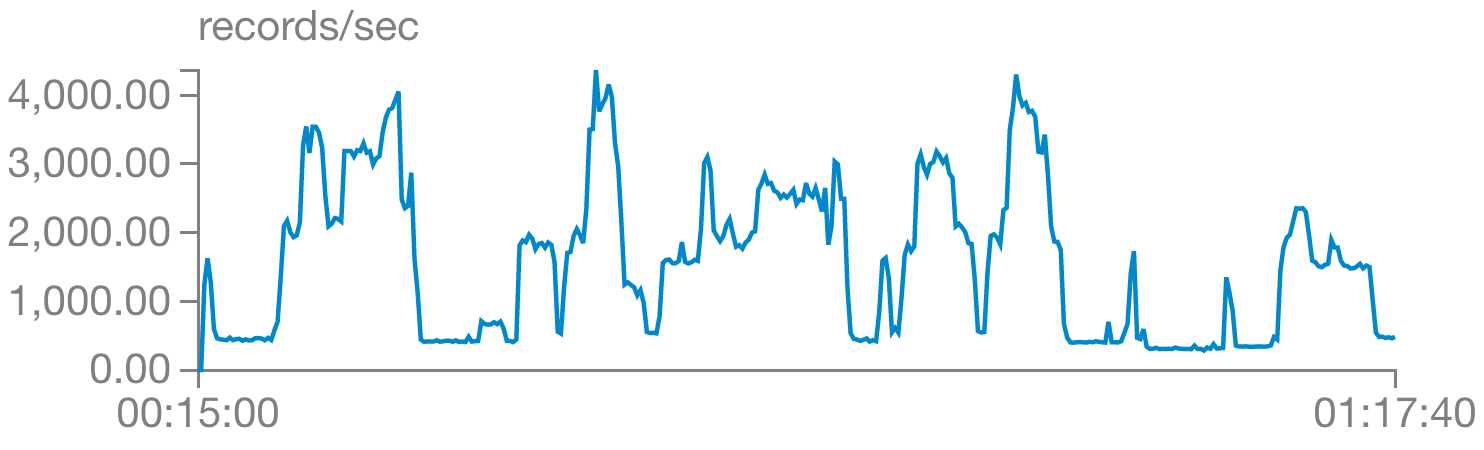
\includegraphics[scale=0.6]{workload1.png}
        \caption{Workload 1}
    \end{subfigure}
    \begin{subfigure}[h]{\linewidth}
        \centering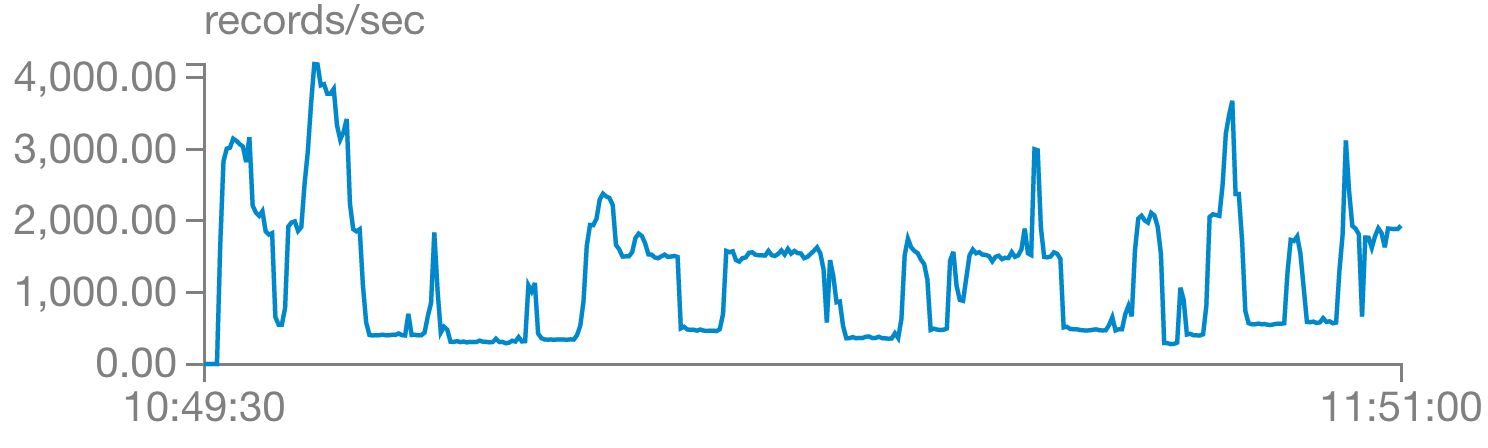
\includegraphics[scale=0.6]{workload2.png}
        \caption{Workload 2}
    \end{subfigure}
    \caption{Two Workloads of DEBS 2014}
    \label{eval:fig:workload}
\end{figure}

The workload involves sensors that measure energy consumption of devices. Each device is connected to one household which in turn is located in one house. This creates a hierarchy from house as parent of households and household as parent of devices. The workload asks to predict energy consumption per device, per household, and per house  for next window of time. The prediction runs over a sliding window of historical measurements which contains $n$ elements. Assuming $window$ variable contains $n$ elements of the history, Equation~\ref{eval:l:pred} defines how the predicted value is calculated.
\begin{equation}
\text{predicted value} = \frac{\text{average(window)} + \text{median(window)}}{2}
\label{eval:l:pred}
\end{equation}

Note that intensity of the workload does not solely depend on number of incoming messages. It also depends on uniqueness of device IDs. A unique device ID inside a micro batch leads to recalculation of Equation~\ref{eval:l:pred} which on its own depends on sort operation to calculate median value. That is, the following cases might occur in one micro batch:
\begin{itemize}
    \item Number of incoming messages is high and uniqueness of devices is also high.
    \item Number if incoming messages is high but uniqueness of devices is low.
    \item Number of incoming messages is low but uniqueness of devices is high.
    \item Number of incoming messages is low and uniqueness of devices is also low.
\end{itemize}
As an example, consider these two batches:
\begin{enumerate}
    \item \label{eval:wl-ex1} A batch of 500 records belonging to 500 hundred devices -- one record for each device -- which leads to 500 sort operations. Bare in mind that, it is \emph{not} 500 hundred sort operation on a 1-element list. Each record is accumulated with previous records of the sliding window and then sorted.
    \item \label{eval:wl-ex2} A batch of 2000 records belonging to 5 devices -- 400 hundred records for each device -- which leads to 5 sort operations.
\end{enumerate}
Case~\ref{eval:wl-ex1} is much more CPU intensive than case~\ref{eval:wl-ex2}. In order to make each workload CPU intensive enough, window size is changed for each workload. Table~\ref{eval:tab:history} defines the history window size for each workload.
\begin{table}[h]
    \begin{tabular}{lc}
        \toprule
        \textbf{Workload} & \textbf{Window Size = $n$ }\\
        \midrule
        Workload 1 & 1650\\
        Workload 2 & 1900\\
        \bottomrule
    \end{tabular}
    \centering
    \caption{Workload Window Size}
    \label{eval:tab:history}
\end{table}

In all experiments \emph{batch size} is set to 10 seconds. The cluster uses 24 executors with minimum of 4 executors that should be respected by Auto-Scaler. All experiments start with minimum number of executors -- 4 in this case -- and run for \emph{one} hour. In case any training is required to run the experiment, training data set is separated from the original workload dataset. In all experiments -- except the last one -- four charts are illustrated. Two charts for latency and two charts for number of executors. Candlestick charts depicts minimum, 10 percentile, average, 90 percentile and maximum values. Furthermore, all experiments were run \emph{two} times and the average of them is included in charts. Note that for the sake of brevity in following experiments W1 stands for Workload 1 and W2 stands for Workload 2.
\clearpage
\section{Experiment 1: Executor Strategy}
This experiment has been designed to illustrate the strategy of adding/removing executors when taking Scale-In or Scale-Out actions. Table~\ref{eval:tab:ex1} shows the configuration of this experiment.
\begin{table}[h]
    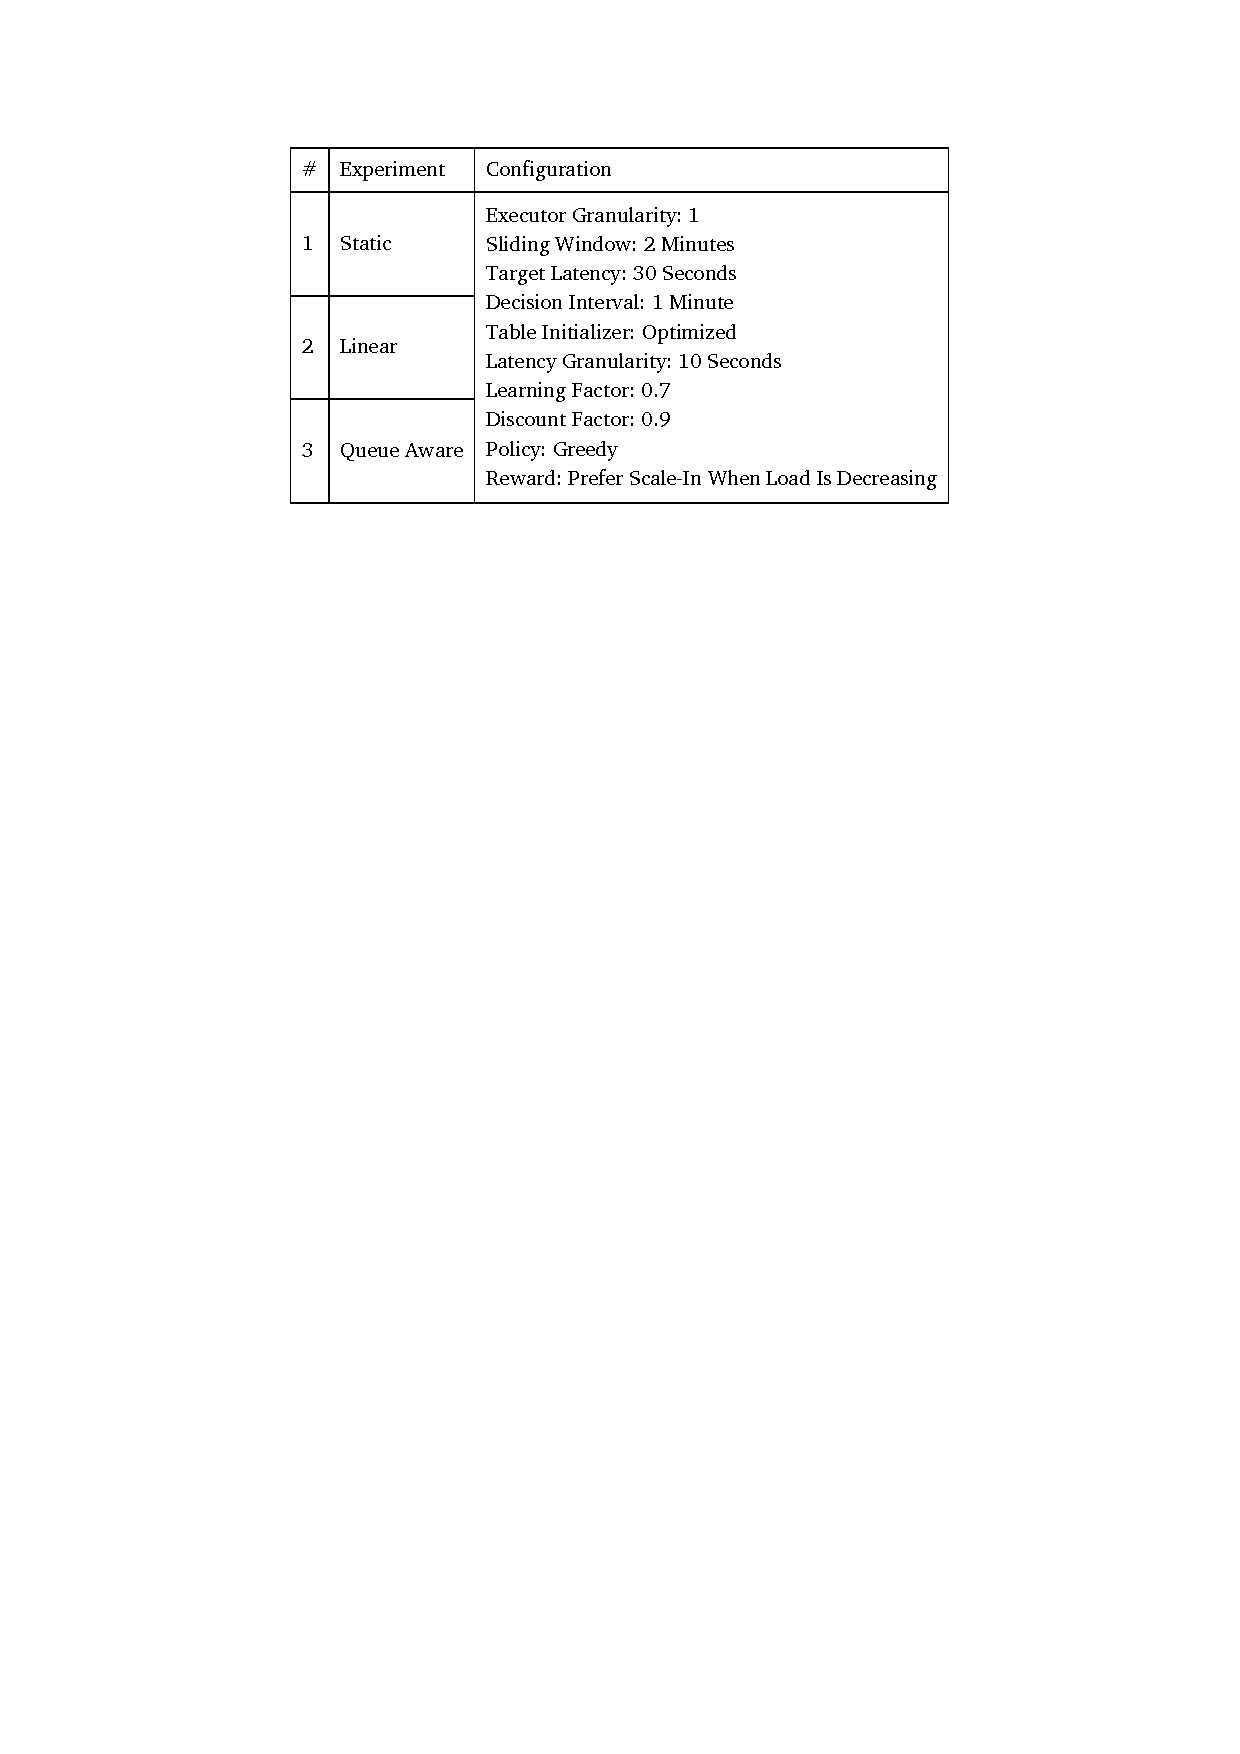
\includegraphics[clip,trim=3.6cm 21.18cm 2.75cm 2.5cm]{tables/ex1.pdf}
    \centering
    \caption{Executor Strategy Configuration Parameters}
    \label{eval:tab:ex1}
\end{table}

Figure~\ref{eval:f:e1:w1:lat},~\ref{eval:f:e1:w1:exec},~\ref{eval:f:e1:w2:lat} and ~\ref{eval:f:e1:w2:exec} depicts detailed latency and executor charts for both workloads. Figure~\ref{eval:f:e1:w1:lat-c},~\ref{eval:f:e1:w1:exec-c},~\ref{eval:f:e1:w2:lat-c} and ~\ref{eval:f:e1:w2:exec-c} illustrates average and percentile charts for both workloads.

\begin{figure}[!htbp]
\centering
\begin{gnuplot}[terminal=epslatex, terminaloptions=color colortext]
set terminal epslatex size 16cm,7.5cm
set key inside center top horizontal box opaque
set datafile separator ';'
set xdata time
set timefmt '%H:%M:%S'
set xr ['0:00:00':'1:00:00']
set yr [0:160]
set xtics '00:00:00',600 nomirror
set ytics 0,30 nomirror
set y2r [0:160]
set y2tics 0,30
set samples 50000 
unset mxtics
unset mytics
set grid ytics lc rgb "#bbbbbb" lw 1 lt 0
set grid xtics lc rgb "#bbbbbb" lw 1 lt 0
unset xl
set yl 'Latency (Seconds)'
plot 'ex/e1/w1/latency.csv' using 1:2 w l lc 'red' lw 4 smooth csplines t 'Static',\
'' using 1:3 w l lc 'blue' lw 4 smooth csplines t 'Linear',\
'' using 1:4 w l lc 'black' lw 4 smooth csplines t 'Q-Aware'
\end{gnuplot}
\caption{Executor Strategy -- W1 -- Latency}
\label{eval:f:e1:w1:lat}
\end{figure}
\clearpage
\begin{figure}[H]
	\centering
	\begin{minipage}[h]{\linewidth}
    	\centering
    	\begin{gnuplot}[terminal=epslatex, terminaloptions=color colortext]
    		set terminal epslatex size 16cm,7.5cm
    		set key inside center top horizontal box opaque
    		set datafile separator ';'
    		set xdata time
    		set timefmt '%H:%M:%S'
    		set xr ['0:00:00':'1:00:00']
    		set yr [2:28]
    		set y2r [2:28]
    		set ytics 0,4 nomirror
    		set xtics '00:00:00',600 nomirror
    		set y2tics 0,4
    		unset mxtics
    		unset mytics
    		unset xl
            set grid ytics lc rgb "#bbbbbb" lw 1 lt 0
            set grid xtics lc rgb "#bbbbbb" lw 1 lt 0
    		set yl 'Number of Executors'
    		plot 'ex/e1/w1/exec.csv' using 1:2 w l lc 'red' lw 4 t 'Static',\
    		'' using 1:3 w l lc 'blue' lw 4 t 'Linear',\
    		'' using 1:4 w l lc 'black' lw 4 t 'Q-Aware'
    	\end{gnuplot}
    	\caption{Executor Strategy -- W1 -- Number of Executors}
    	\label{eval:f:e1:w1:exec}
	\end{minipage}\hfil
	\begin{minipage}[h]{\linewidth}
        \centering
        \begin{gnuplot}[terminal=epslatex, terminaloptions=color colortext]
            set terminal epslatex size 16cm,7.5cm
            set key inside center top horizontal box opaque
            set datafile separator ';'
            set xdata time
            set timefmt '%H:%M:%S'
            set xr ['0:00:00':'1:00:00']
            set yr [0:180]
            set y2r [0:180]
            set xtics '00:00:00',600 nomirror
            set ytics 0,30 nomirror
            set y2tics 0,30
            unset mxtics
            unset mytics
            set samples 50000 
            unset xl
            set grid ytics lc rgb "#bbbbbb" lw 1 lt 0
            set grid xtics lc rgb "#bbbbbb" lw 1 lt 0
            set yl 'Latency (Seconds)'
            plot 'ex/e1/w2/latency.csv' using 1:2 w l lc 'red' lw 4 smooth csplines t 'Static',\
            '' using 1:3 w l lc 'blue' lw 4 smooth csplines t 'Linear',\
            '' using 1:4 w l lc 'black' lw 4 smooth csplines t 'Q-Aware'
        \end{gnuplot}
        \caption{Executor Strategy -- W2 -- Latency}
        \label{eval:f:e1:w2:lat}
    \end{minipage}\hfil
    	\begin{minipage}[h]{\linewidth}
        \centering
        \begin{gnuplot}[terminal=epslatex, terminaloptions=color colortext]
            set terminal epslatex size 16cm,7.5cm
            set key inside center top horizontal box opaque
            set datafile separator ';'
            set xdata time
            set timefmt '%H:%M:%S'
            set xr ['0:00:00':'1:00:00']
            set yr [2:28]
            set y2r [2:28]
            set xtics '00:00:00',600 nomirror
            set ytics 0,4 nomirror
            set y2tics 0,4
            unset mxtics
            unset mytics
            unset xl
            set grid ytics lc rgb "#bbbbbb" lw 1 lt 0
            set grid xtics lc rgb "#bbbbbb" lw 1 lt 0
            set yl 'Number of Executors'
            plot 'ex/e1/w2/exec.csv' using 1:2 w l lc 'red' lw 4 t 'Static',\
            '' using 1:3 w l lc 'blue' lw 4 t 'Linear',\
            '' using 1:4 w l lc 'black' lw 4 t 'Q-Aware'
        \end{gnuplot}
        \caption{Executor Strategy -- W2 -- Number of Executors}
        \label{eval:f:e1:w2:exec}
    \end{minipage}
\end{figure}
\clearpage
\begin{figure}[H]
	\centering
    \begin{minipage}[h]{0.5\linewidth}
        \centering
        \begin{gnuplot}[terminal=epslatex, terminaloptions=color colortext]
            set terminal epslatex size 9cm,6cm
            set key inside center top horizontal box opaque
            set datafile separator ';'
            set xr [0.5:3.5]
            set yr [0:210]
            set ytics 0,30
            unset y2r
            unset y2tics
            set boxwidth 0.3 absolute
            set style fill empty
            unset xl
            set grid ytics lc rgb "#bbbbbb" lw 1 lt 0
            set grid xtics lc rgb "#bbbbbb" lw 1 lt 0
            set yl 'Latency (Seconds)'
            plot 'ex/e1/w1/latency-c.csv' using 1:2:3:4:5:xticlabels(7) with candlesticks lc 'black' lw 4 t 'Min/Max/Percentiles',\
            '' using 1:6:6:6:6 with linespoints pt 5 lc 'black' lw 4 t 'Average',\
            30 dashtype 2 lc 'black' lw 4 t 'Target'
        \end{gnuplot}
        \caption{Executor Strategy -- W1 -- Latency}
        \label{eval:f:e1:w1:lat-c}
    \end{minipage}\hfil
    \begin{minipage}[h]{0.5\linewidth}
        \centering
        \begin{gnuplot}[terminal=epslatex, terminaloptions=color colortext]
            set terminal epslatex size 9cm,6cm
            set key inside center top horizontal box opaque
            set datafile separator ';'
            set xr [0.5:3.5]
            set yr [2:32]
            set ytics 0,4
            unset y2r
            unset y2tics
            set boxwidth 0.3 absolute
            set style fill empty
            unset xl
            set grid ytics lc rgb "#bbbbbb" lw 1 lt 0
            set grid xtics lc rgb "#bbbbbb" lw 1 lt 0
            set yl 'Number of Executors'
            plot 'ex/e1/w1/exec-c.csv' using 1:2:3:4:5:xticlabels(7) with candlesticks lc 'black' lw 4 t 'Min/Max/Percentiles',\
            '' using 1:6:6:6:6 with linespoints pt 5 lc 'black' lw 4 t 'Average' 
        \end{gnuplot}
        \caption{Executor Strategy -- W1 -- Number of Executors}
        \label{eval:f:e1:w1:exec-c}
    \end{minipage}
	\begin{minipage}[h]{0.5\linewidth}
		\centering
		\begin{gnuplot}[terminal=epslatex, terminaloptions=color colortext]
			set terminal epslatex size 9cm,6cm
			set key inside center top horizontal box opaque
			set datafile separator ';'
			set xr [0.5:3.5]
			set yr [0:230]
			set ytics 0,30
            unset y2r
			unset y2tics
			set boxwidth 0.3 absolute
			set style fill empty
			unset xl
            set grid ytics lc rgb "#bbbbbb" lw 1 lt 0
            set grid xtics lc rgb "#bbbbbb" lw 1 lt 0
			set yl 'Latency (Seconds)'
			plot 'ex/e1/w2/latency-c.csv' using 1:2:3:4:5:xticlabels(7) with candlesticks lc 'black' lw 4 t 'Min/Max/Percentiles',\
			'' using 1:6:6:6:6 with linespoints pt 5 lc 'black' lw 4 t 'Average',\
            30 dashtype 2 lc 'black' lw 4 t 'Target'
		\end{gnuplot}
		\caption{Executor Strategy -- W2 -- Latency}
		\label{eval:f:e1:w2:lat-c}
	\end{minipage}\hfil
    \begin{minipage}[h]{0.5\linewidth}
        \centering
        \begin{gnuplot}[terminal=epslatex, terminaloptions=color colortext]
            set terminal epslatex size 9cm,6cm
            set key inside center top horizontal box opaque
            set datafile separator ';'
            set xr [0.5:3.5]
            set yr [2:32]
            set ytics 0,4
            unset y2r
            unset y2tics
            set boxwidth 0.3 absolute
            set style fill empty
            unset xl
            set grid ytics lc rgb "#bbbbbb" lw 1 lt 0
            set grid xtics lc rgb "#bbbbbb" lw 1 lt 0
            set yl 'Number of Executors'
            plot 'ex/e1/w2/exec-c.csv' using 1:2:3:4:5:xticlabels(7) with candlesticks lc 'black' lw 4 t 'Min/Max/Percentiles','' using 1:6:6:6:6 with linespoints pt 5 lc 'black' lw 4 t 'Average' 
        \end{gnuplot}
        \caption{Executor Strategy -- W2 -- Number of Executors}
        \label{eval:f:e1:w2:exec-c}
    \end{minipage}
\end{figure}
A possible conclusion would be that Queue Aware strategy is the best strategy amongst three strategies. However, it can't be proven now. More experiments shall be done. Thus, for next set of experiments Queue Aware strategy is chosen to be evaluated extensively.
\clearpage
\section{Experiment 2: History Window}
This experiment has been designed to illustrate the effect of history window on quality of decision made by Auto-Scaler. Table~\ref{eval:tab:ex2} shows the configuration of this experiment.
\begin{table}[h]
    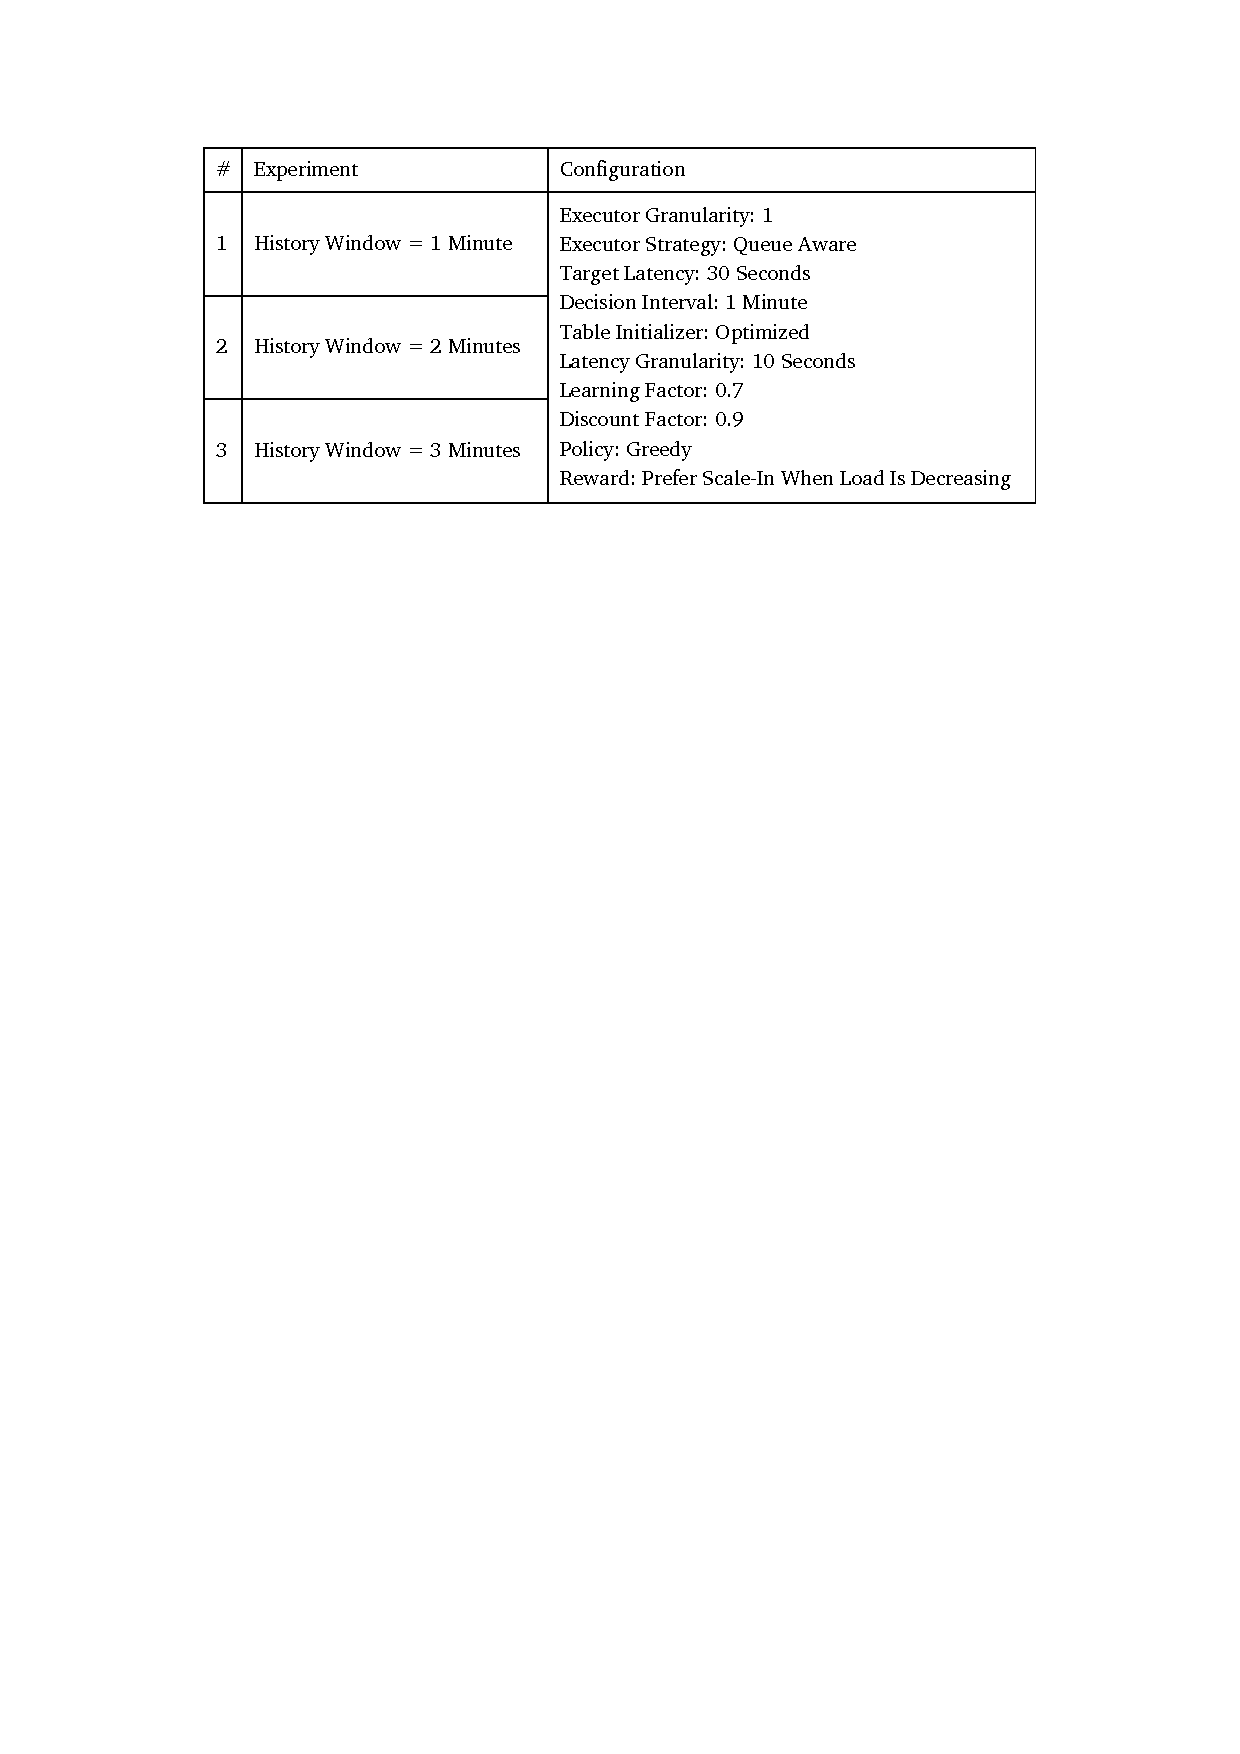
\includegraphics[clip,trim=3.3cm 21.18cm 3.25cm 2.5cm]{tables/ex2.pdf}
    \centering
    \caption{History Window Configuration Parameters}
    \label{eval:tab:ex2}
\end{table}

Figure~\ref{eval:f:e2:w1:lat},~\ref{eval:f:e2:w1:exec},~\ref{eval:f:e2:w2:lat} and ~\ref{eval:f:e2:w2:exec} depicts detailed latency and executor charts for both workloads. Figure~\ref{eval:f:e2:w1:lat-c},~\ref{eval:f:e2:w1:exec-c},~\ref{eval:f:e2:w2:lat-c} and ~\ref{eval:f:e2:w2:exec-c} illustrates average and percentile charts for both workloads.

\begin{figure}[!htbp]
    \centering
    \begin{gnuplot}[terminal=epslatex, terminaloptions=color colortext]
        set terminal epslatex size 16cm,7.5cm
        set key inside center top horizontal box opaque
        set datafile separator ';'
        set xdata time
        set timefmt '%H:%M:%S'
        set xr ['0:00:00':'1:00:00']
        set yr [0:120]
        set xtics '00:00:00',600 nomirror
        set ytics 0,30 nomirror
        set y2r [0:120]
        set y2tics 0,30
        set samples 50000 
        unset mxtics
        unset mytics
        set grid ytics lc rgb "#bbbbbb" lw 1 lt 0
        set grid xtics lc rgb "#bbbbbb" lw 1 lt 0
        unset xl
        set yl 'Latency (Seconds)'
        plot 'ex/e2/w1/latency.csv' using 1:2 w l lc 'red' lw 4 smooth csplines t '1 Min',\
        '' using 1:3 w l lc 'blue' lw 4 smooth csplines t '2 Min',\
        '' using 1:4 w l lc 'black' lw 4 smooth csplines t '3 Min'
    \end{gnuplot}
    \caption{History Window -- W1 -- Latency}
    \label{eval:f:e2:w1:lat}
\end{figure}
\clearpage
\begin{figure}[H]
    \centering
    \begin{minipage}[h]{\linewidth}
        \centering
        \begin{gnuplot}[terminal=epslatex, terminaloptions=color colortext]
            set terminal epslatex size 16cm,7.5cm
            set key inside center top horizontal box opaque
            set datafile separator ';'
            set xdata time
            set timefmt '%H:%M:%S'
            set xr ['0:00:00':'1:00:00']
            set yr [2:28]
            set y2r [2:28]
            set ytics 0,4 nomirror
            set xtics '00:00:00',600 nomirror
            set y2tics 0,4
            unset mxtics
            unset mytics
            unset xl
            set grid ytics lc rgb "#bbbbbb" lw 1 lt 0
            set grid xtics lc rgb "#bbbbbb" lw 1 lt 0
            set yl 'Number of Executors'
            plot 'ex/e2/w1/exec.csv' using 1:2 w l lc 'red' lw 4 t '1 Min',\
            '' using 1:3 w l lc 'blue' lw 4 t '2 Min',\
            '' using 1:4 w l lc 'black' lw 4 t '3 Min'
        \end{gnuplot}
        \caption{History Window -- W1 -- Number of Executors}
        \label{eval:f:e2:w1:exec}
    \end{minipage}\hfil
    \begin{minipage}[h]{\linewidth}
        \centering
        \begin{gnuplot}[terminal=epslatex, terminaloptions=color colortext]
            set terminal epslatex size 16cm,7.5cm
            set key inside center top horizontal box opaque
            set datafile separator ';'
            set xdata time
            set timefmt '%H:%M:%S'
            set xr ['0:00:00':'1:00:00']
            set yr [0:150]
            set y2r [0:150]
            set xtics '00:00:00',600 nomirror
            set ytics 0,30 nomirror
            set y2tics 0,30
            unset mxtics
            unset mytics
            set samples 50000 
            unset xl
            set grid ytics lc rgb "#bbbbbb" lw 1 lt 0
            set grid xtics lc rgb "#bbbbbb" lw 1 lt 0
            set yl 'Latency (Seconds)'
            plot 'ex/e2/w2/latency.csv' using 1:2 w l lc 'red' lw 4 smooth csplines t '1 Min',\
            '' using 1:3 w l lc 'blue' lw 4 smooth csplines t '2 Min',\
            '' using 1:4 w l lc 'black' lw 4 smooth csplines t '3 Min'
        \end{gnuplot}
        \caption{History Window -- W2 -- Latency}
        \label{eval:f:e2:w2:lat}
    \end{minipage}\hfil
    \begin{minipage}[h]{\linewidth}
        \centering
        \begin{gnuplot}[terminal=epslatex, terminaloptions=color colortext]
            set terminal epslatex size 16cm,7.5cm
            set key inside center top horizontal box opaque
            set datafile separator ';'
            set xdata time
            set timefmt '%H:%M:%S'
            set xr ['0:00:00':'1:00:00']
            set yr [2:28]
            set y2r [2:28]
            set xtics '00:00:00',600 nomirror
            set ytics 0,4 nomirror
            set y2tics 0,4
            unset mxtics
            unset mytics
            unset xl
            set grid ytics lc rgb "#bbbbbb" lw 1 lt 0
            set grid xtics lc rgb "#bbbbbb" lw 1 lt 0
            set yl 'Number of Executors'
            plot 'ex/e2/w2/exec.csv' using 1:2 w l lc 'red' lw 4 t '1 Min',\
            '' using 1:3 w l lc 'blue' lw 4 t '2 Min',\
            '' using 1:4 w l lc 'black' lw 4 t '3 Min'
        \end{gnuplot}
        \caption{History Window -- W2 -- Number of Executors}
        \label{eval:f:e2:w2:exec}
    \end{minipage}
\end{figure}
\clearpage
\begin{figure}[H]
    \centering
    \begin{minipage}[h]{0.5\linewidth}
        \centering
        \begin{gnuplot}[terminal=epslatex, terminaloptions=color colortext]
            set terminal epslatex size 9cm,6cm
            set key inside center top horizontal box opaque
            set datafile separator ';'
            set xr [0.5:3.5]
            set yr [0:150]
            set ytics 0,30
            unset y2r
            unset y2tics
            set boxwidth 0.3 absolute
            set style fill empty
            unset xl
            set grid ytics lc rgb "#bbbbbb" lw 1 lt 0
            set grid xtics lc rgb "#bbbbbb" lw 1 lt 0
            set yl 'Latency (Seconds)'
            plot 'ex/e2/w1/latency-c.csv' using 1:2:3:4:5:xticlabels(7) with candlesticks lc 'black' lw 4 t 'Min/Max/Percentiles',\
            '' using 1:6:6:6:6 with linespoints pt 5 lc 'black' lw 4 t 'Average',\
            30 dashtype 2 lc 'black' lw 4 t 'Target'
        \end{gnuplot}
        \caption{History Window -- W1 -- Latency}
        \label{eval:f:e2:w1:lat-c}
    \end{minipage}\hfil
    \begin{minipage}[h]{0.5\linewidth}
        \centering
        \begin{gnuplot}[terminal=epslatex, terminaloptions=color colortext]
            set terminal epslatex size 9cm,6cm
            set key inside center top horizontal box opaque
            set datafile separator ';'
            set xr [0.5:3.5]
            set yr [2:32]
            set ytics 0,4
            unset y2r
            unset y2tics
            set boxwidth 0.3 absolute
            set style fill empty
            unset xl
            set grid ytics lc rgb "#bbbbbb" lw 1 lt 0
            set grid xtics lc rgb "#bbbbbb" lw 1 lt 0
            set yl 'Number of Executors'
            plot 'ex/e2/w1/exec-c.csv' using 1:2:3:4:5:xticlabels(7) with candlesticks lc 'black' lw 4 t 'Min/Max/Percentiles',\
            '' using 1:6:6:6:6 with linespoints pt 5 lc 'black' lw 4 t 'Average' 
        \end{gnuplot}
        \caption{History Window -- W1 -- Number of Executors}
        \label{eval:f:e2:w1:exec-c}
    \end{minipage}
    \begin{minipage}[h]{0.5\linewidth}
        \centering
        \begin{gnuplot}[terminal=epslatex, terminaloptions=color colortext]
            set terminal epslatex size 9cm,6cm
            set key inside center top horizontal box opaque
            set datafile separator ';'
            set xr [0.5:3.5]
            set yr [0:180]
            set ytics 0,30
            unset y2r
            unset y2tics
            set boxwidth 0.3 absolute
            set style fill empty
            unset xl
            set grid ytics lc rgb "#bbbbbb" lw 1 lt 0
            set grid xtics lc rgb "#bbbbbb" lw 1 lt 0
            set yl 'Latency (Seconds)'
            plot 'ex/e2/w2/latency-c.csv' using 1:2:3:4:5:xticlabels(7) with candlesticks lc 'black' lw 4 t 'Min/Max/Percentiles',\
            '' using 1:6:6:6:6 with linespoints pt 5 lc 'black' lw 4 t 'Average',\
            30 dashtype 2 lc 'black' lw 4 t 'Target'
        \end{gnuplot}
        \caption{History Window -- W2 -- Latency}
        \label{eval:f:e2:w2:lat-c}
    \end{minipage}\hfil
    \begin{minipage}[h]{0.5\linewidth}
        \centering
        \begin{gnuplot}[terminal=epslatex, terminaloptions=color colortext]
            set terminal epslatex size 9cm,6cm
            set key inside center top horizontal box opaque
            set datafile separator ';'
            set xr [0.5:3.5]
            set yr [2:32]
            set ytics 0,4
            unset y2r
            unset y2tics
            set boxwidth 0.3 absolute
            set style fill empty
            unset xl
            set grid ytics lc rgb "#bbbbbb" lw 1 lt 0
            set grid xtics lc rgb "#bbbbbb" lw 1 lt 0
            set yl 'Number of Executors'
            plot 'ex/e2/w2/exec-c.csv' using 1:2:3:4:5:xticlabels(7) with candlesticks lc 'black' lw 4 t 'Min/Max/Percentiles','' using 1:6:6:6:6 with linespoints pt 5 lc 'black' lw 4 t 'Average' 
        \end{gnuplot}
        \caption{History Window -- W2 -- Number of Executors}
        \label{eval:f:e2:w2:exec-c}
    \end{minipage}
\end{figure}

Note that, short history window (like one-minute) makes Auto-Scaler too sensitive to noisy workloads. This can be confirmed by Figure~\ref{eval:f:e2:w2:exec}. As depicted, one-minute history window suffers from zig-zag decisions when it reaches 24 executors. Two-minute window to some degree suffers from this issue as well. However, three-minute window is resistant to this issue. In general, history window of two minutes shows better results than the others. Thus, for rest of the experiments this window size will be used.
\clearpage
\section{Experiment 3: Decision Interval}
The Auto-Scaler implemented in thesis makes decisions in intervals defined by \lstinline|decisionInterval| parameter. This experiment has been designed to illustrate the effect of this parameter on behavior of the Auto-Scaler. Table~\ref{eval:tab:ex3} shows the configuration of this experiment.
\begin{table}[h]
    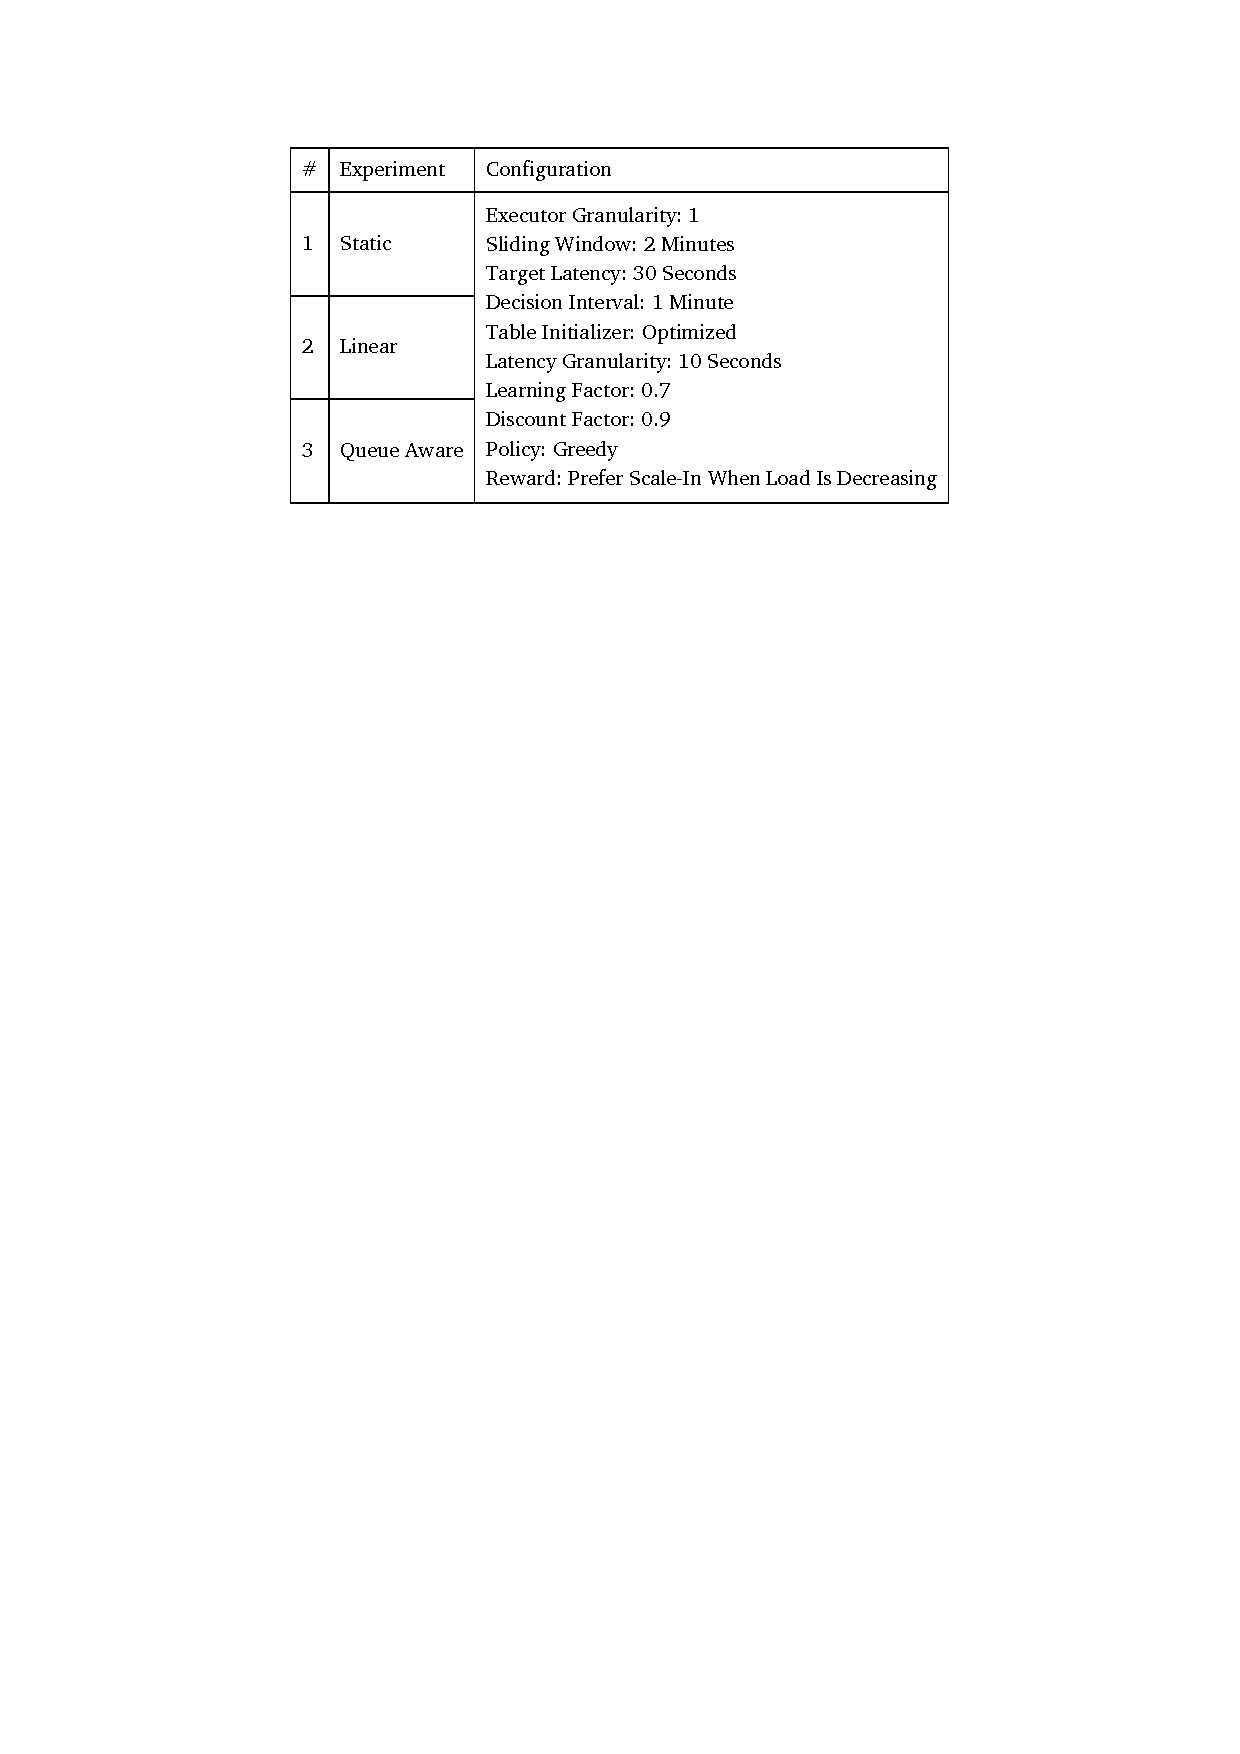
\includegraphics[clip,trim=3.3cm 21.18cm 3.25cm 2.5cm]{tables/ex3.pdf}
    \centering
    \caption{Decision Interval Configuration Parameters}
    \label{eval:tab:ex3}
\end{table}

Figure~\ref{eval:f:e3:w1:lat},~\ref{eval:f:e3:w1:exec},~\ref{eval:f:e3:w2:lat} and ~\ref{eval:f:e3:w2:exec} depicts detailed latency and executor charts for both workloads. Figure~\ref{eval:f:e3:w1:lat-c},~\ref{eval:f:e3:w1:exec-c},~\ref{eval:f:e3:w2:lat-c} and ~\ref{eval:f:e3:w2:exec-c} illustrates average and percentile charts for both workloads.

\begin{figure}[!htbp]
    \centering
    \begin{gnuplot}[terminal=epslatex, terminaloptions=color colortext]
        set terminal epslatex size 16cm,7.5cm
        set key inside center top horizontal box opaque
        set datafile separator ';'
        set xdata time
        set timefmt '%H:%M:%S'
        set xr ['0:00:00':'1:00:00']
        set yr [0:120]
        set xtics '00:00:00',600 nomirror
        set ytics 0,30 nomirror
        set y2r [0:120]
        set y2tics 0,30
        set samples 50000 
        unset mxtics
        unset mytics
        set grid ytics lc rgb "#bbbbbb" lw 1 lt 0
        set grid xtics lc rgb "#bbbbbb" lw 1 lt 0
        unset xl
        set yl 'Latency (Seconds)'
        plot 'ex/e3/w1/latency.csv' using 1:2 w l lc 'red' lw 4 smooth csplines t '1 Min',\
        '' using 1:3 w l lc 'blue' lw 4 smooth csplines t '2 Min',\
        '' using 1:4 w l lc 'black' lw 4 smooth csplines t '3 Min'
    \end{gnuplot}
    \caption{Decision Interval -- W1 -- Latency}
    \label{eval:f:e3:w1:lat}
\end{figure}
\clearpage
\begin{figure}[H]
    \centering
    \begin{minipage}[h]{\linewidth}
        \centering
        \begin{gnuplot}[terminal=epslatex, terminaloptions=color colortext]
            set terminal epslatex size 16cm,7.5cm
            set key inside center top horizontal box opaque
            set datafile separator ';'
            set xdata time
            set timefmt '%H:%M:%S'
            set xr ['0:00:00':'1:00:00']
            set yr [2:28]
            set y2r [2:28]
            set ytics 0,4 nomirror
            set xtics '00:00:00',600 nomirror
            set y2tics 0,4
            unset mxtics
            unset mytics
            unset xl
            set grid ytics lc rgb "#bbbbbb" lw 1 lt 0
            set grid xtics lc rgb "#bbbbbb" lw 1 lt 0
            set yl 'Number of Executors'
            plot 'ex/e3/w1/exec.csv' using 1:2 w l lc 'red' lw 4 t '1 Min',\
            '' using 1:3 w l lc 'blue' lw 4 t '2 Min',\
            '' using 1:4 w l lc 'black' lw 4 t '3 Min'
        \end{gnuplot}
        \caption{Decision Interval -- W1 -- Number of Executors}
        \label{eval:f:e3:w1:exec}
    \end{minipage}\hfil
    \begin{minipage}[h]{\linewidth}
        \centering
        \begin{gnuplot}[terminal=epslatex, terminaloptions=color colortext]
            set terminal epslatex size 16cm,7.5cm
            set key inside center top horizontal box opaque
            set datafile separator ';'
            set xdata time
            set timefmt '%H:%M:%S'
            set xr ['0:00:00':'1:00:00']
            set yr [0:150]
            set y2r [0:150]
            set xtics '00:00:00',600 nomirror
            set ytics 0,30 nomirror
            set y2tics 0,30
            unset mxtics
            unset mytics
            set samples 50000 
            unset xl
            set grid ytics lc rgb "#bbbbbb" lw 1 lt 0
            set grid xtics lc rgb "#bbbbbb" lw 1 lt 0
            set yl 'Latency (Seconds)'
            plot 'ex/e3/w2/latency.csv' using 1:2 w l lc 'red' lw 4 smooth csplines t '1 Min',\
            '' using 1:3 w l lc 'blue' lw 4 smooth csplines t '2 Min',\
            '' using 1:4 w l lc 'black' lw 4 smooth csplines t '3 Min'
        \end{gnuplot}
        \caption{Decision Interval -- W2 -- Latency}
        \label{eval:f:e3:w2:lat}
    \end{minipage}\hfil
    \begin{minipage}[h]{\linewidth}
        \centering
        \begin{gnuplot}[terminal=epslatex, terminaloptions=color colortext]
            set terminal epslatex size 16cm,7.5cm
            set key inside center top horizontal box opaque
            set datafile separator ';'
            set xdata time
            set timefmt '%H:%M:%S'
            set xr ['0:00:00':'1:00:00']
            set yr [2:28]
            set y2r [2:28]
            set xtics '00:00:00',600 nomirror
            set ytics 0,4 nomirror
            set y2tics 0,4
            unset mxtics
            unset mytics
            unset xl
            set grid ytics lc rgb "#bbbbbb" lw 1 lt 0
            set grid xtics lc rgb "#bbbbbb" lw 1 lt 0
            set yl 'Number of Executors'
            plot 'ex/e3/w2/exec.csv' using 1:2 w l lc 'red' lw 4 t '1 Min',\
            '' using 1:3 w l lc 'blue' lw 4 t '2 Min',\
            '' using 1:4 w l lc 'black' lw 4 t '3 Min'
        \end{gnuplot}
        \caption{Decision Interval -- W2 -- Number of Executors}
        \label{eval:f:e3:w2:exec}
    \end{minipage}
\end{figure}
\clearpage
\begin{figure}[H]
    \centering
    \begin{minipage}[h]{0.5\linewidth}
        \centering
        \begin{gnuplot}[terminal=epslatex, terminaloptions=color colortext]
            set terminal epslatex size 9cm,6cm
            set key inside center top horizontal box opaque
            set datafile separator ';'
            set xr [0.5:3.5]
            set yr [0:140]
            set ytics 0,30
            unset y2r
            unset y2tics
            set boxwidth 0.3 absolute
            set style fill empty
            unset xl
            set grid ytics lc rgb "#bbbbbb" lw 1 lt 0
            set grid xtics lc rgb "#bbbbbb" lw 1 lt 0
            set yl 'Latency (Seconds)'
            plot 'ex/e3/w1/latency-c.csv' using 1:2:3:4:5:xticlabels(7) with candlesticks lc 'black' lw 4 t 'Min/Max/Percentiles',\
            '' using 1:6:6:6:6 with linespoints pt 5 lc 'black' lw 4 t 'Average',\
            30 dashtype 2 lc 'black' lw 4 t 'Target'
        \end{gnuplot}
        \caption{Decision Interval -- W1 -- Latency}
        \label{eval:f:e3:w1:lat-c}
    \end{minipage}\hfil
    \begin{minipage}[h]{0.5\linewidth}
        \centering
        \begin{gnuplot}[terminal=epslatex, terminaloptions=color colortext]
            set terminal epslatex size 9cm,6cm
            set key inside center top horizontal box opaque
            set datafile separator ';'
            set xr [0.5:3.5]
            set yr [2:32]
            set ytics 0,4
            unset y2r
            unset y2tics
            set boxwidth 0.3 absolute
            set style fill empty
            unset xl
            set grid ytics lc rgb "#bbbbbb" lw 1 lt 0
            set grid xtics lc rgb "#bbbbbb" lw 1 lt 0
            set yl 'Number of Executors'
            plot 'ex/e3/w1/exec-c.csv' using 1:2:3:4:5:xticlabels(7) with candlesticks lc 'black' lw 4 t 'Min/Max/Percentiles',\
            '' using 1:6:6:6:6 with linespoints pt 5 lc 'black' lw 4 t 'Average' 
        \end{gnuplot}
        \caption{Decision Interval -- W1 -- Number of Executors}
        \label{eval:f:e3:w1:exec-c}
    \end{minipage}
    \begin{minipage}[h]{0.5\linewidth}
        \centering
        \begin{gnuplot}[terminal=epslatex, terminaloptions=color colortext]
            set terminal epslatex size 9cm,6cm
            set key inside center top horizontal box opaque
            set datafile separator ';'
            set xr [0.5:3.5]
            set yr [0:180]
            set ytics 0,30
            unset y2r
            unset y2tics
            set boxwidth 0.3 absolute
            set style fill empty
            unset xl
            set grid ytics lc rgb "#bbbbbb" lw 1 lt 0
            set grid xtics lc rgb "#bbbbbb" lw 1 lt 0
            set yl 'Latency (Seconds)'
            plot 'ex/e3/w2/latency-c.csv' using 1:2:3:4:5:xticlabels(7) with candlesticks lc 'black' lw 4 t 'Min/Max/Percentiles',\
            '' using 1:6:6:6:6 with linespoints pt 5 lc 'black' lw 4 t 'Average',\
            30 dashtype 2 lc 'black' lw 4 t 'Target'
        \end{gnuplot}
        \caption{Decision Interval -- W2 -- Latency}
        \label{eval:f:e3:w2:lat-c}
    \end{minipage}\hfil
    \begin{minipage}[h]{0.5\linewidth}
        \centering
        \begin{gnuplot}[terminal=epslatex, terminaloptions=color colortext]
            set terminal epslatex size 9cm,6cm
            set key inside center top horizontal box opaque
            set datafile separator ';'
            set xr [0.5:3.5]
            set yr [2:32]
            set ytics 0,4
            unset y2r
            unset y2tics
            set boxwidth 0.3 absolute
            set style fill empty
            unset xl
            set grid ytics lc rgb "#bbbbbb" lw 1 lt 0
            set grid xtics lc rgb "#bbbbbb" lw 1 lt 0
            set yl 'Number of Executors'
            plot 'ex/e3/w2/exec-c.csv' using 1:2:3:4:5:xticlabels(7) with candlesticks lc 'black' lw 4 t 'Min/Max/Percentiles','' using 1:6:6:6:6 with linespoints pt 5 lc 'black' lw 4 t 'Average' 
        \end{gnuplot}
        \caption{Decision Interval -- W2 -- Number of Executors}
        \label{eval:f:e3:w2:exec-c}
    \end{minipage}
\end{figure}

At this point selecting the best configuration becomes more difficult. Note that two and three-minute decision intervals perform extremely well for Workload 1 and poor for Workload 2. On the other hand one-minute decision interval performs reasonable in both workloads. Thus, this configuration is still preferred.

\clearpage
\section{Experiment 4: State Space Initializer}
As mentioned in Section~\ref{design}, in order to speedup learning process, state space can be initialized using different techniques. This experiment has been designed to illustrate the effect of different state space initializers. In particular, it evaluates effectiveness of optimized initializer in comparison to random and zero initializers. Table~\ref{eval:tab:ex4} shows the configuration of this experiment. Note that, Queue Aware executor strategy is optimized to complement Auto-Scaler's decisions. In order to eliminate positive effect of Queue Aware strategy, Static strategy is used instead to better illustrate the negative effects of random actions.
\begin{table}[h]
    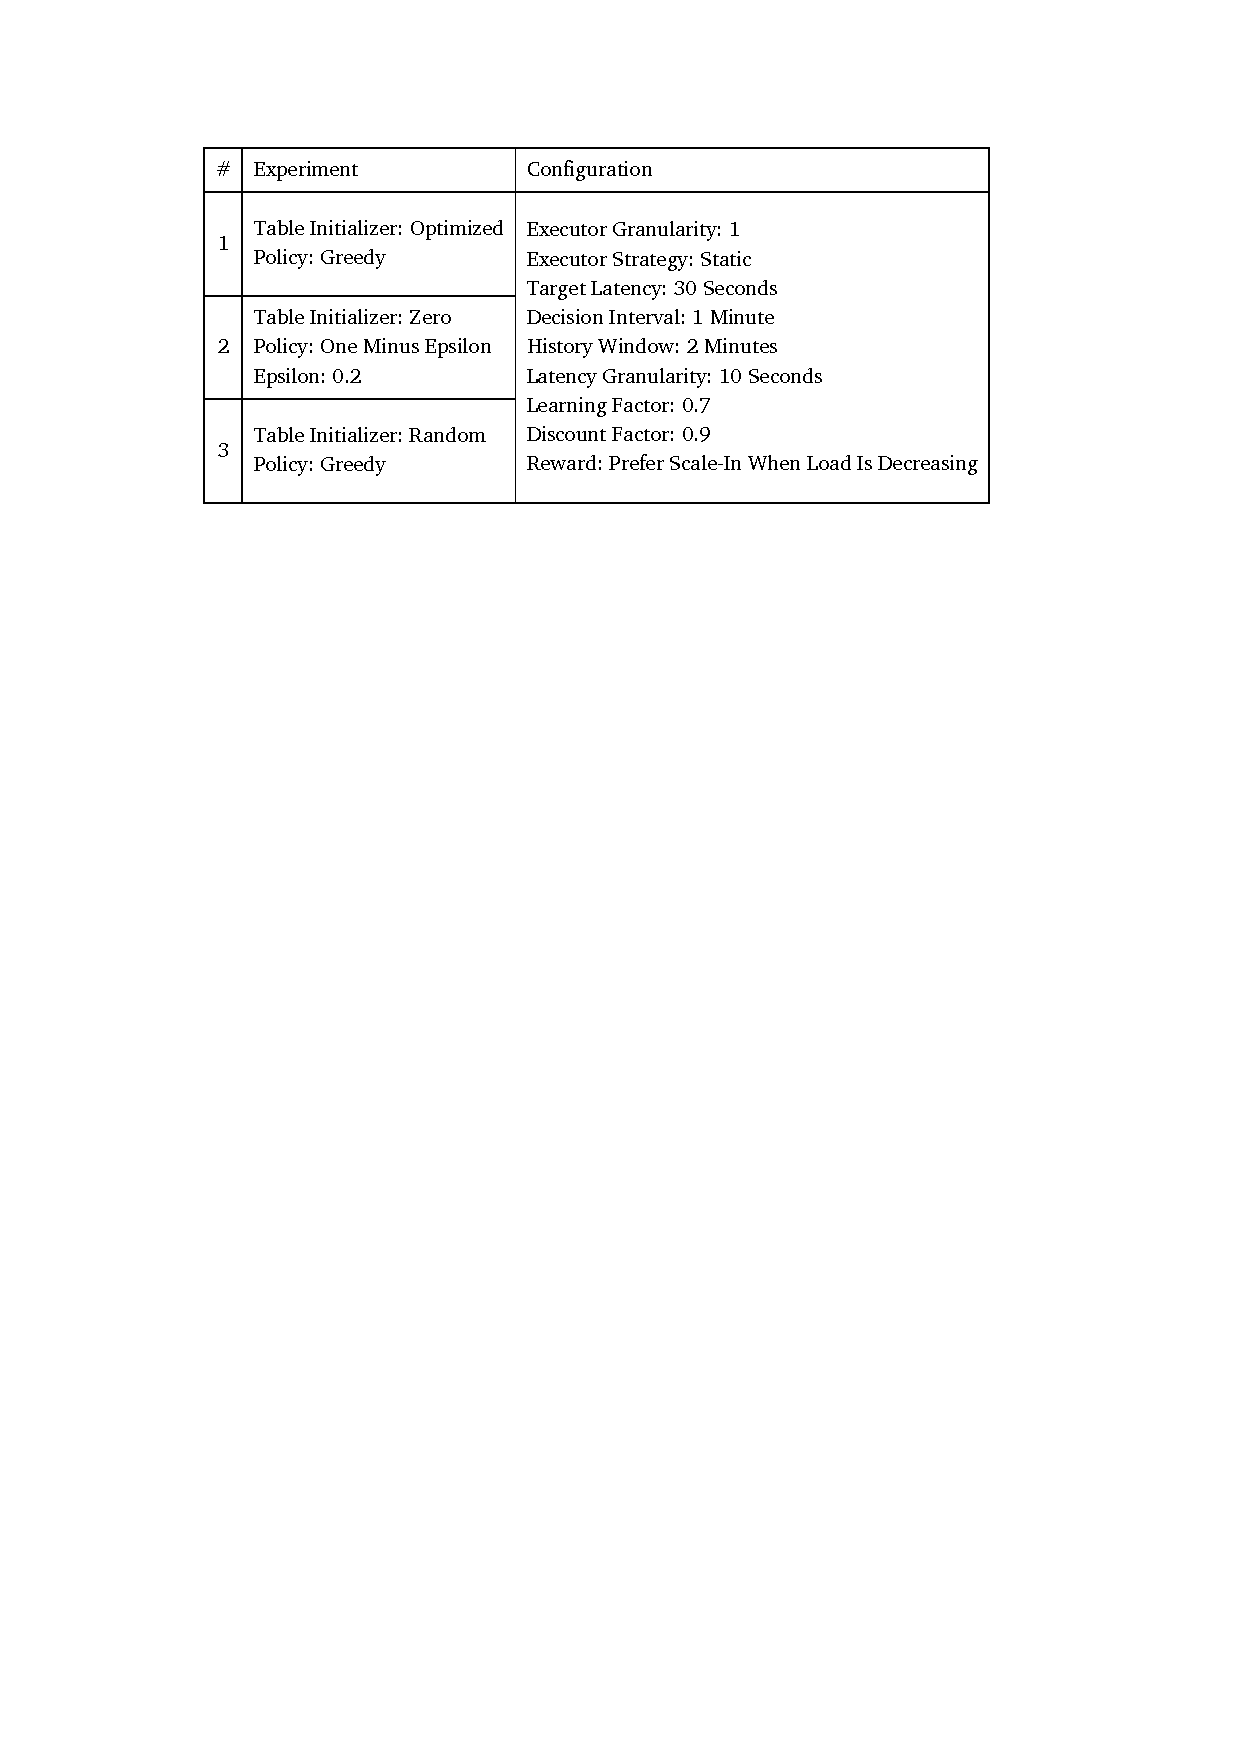
\includegraphics[clip,trim=3.3cm 21.18cm 4.1cm 2.5cm]{tables/ex4.pdf}
    \centering
    \caption{State Space Initializer Configuration Parameters}
    \label{eval:tab:ex4}
\end{table}

Figure~\ref{eval:f:e4:w1:lat},~\ref{eval:f:e4:w1:exec},~\ref{eval:f:e4:w2:lat} and ~\ref{eval:f:e4:w2:exec} depicts detailed latency and executor charts for both workloads. Figure~\ref{eval:f:e4:w1:lat-c},~\ref{eval:f:e4:w1:exec-c},~\ref{eval:f:e4:w2:lat-c} and ~\ref{eval:f:e4:w2:exec-c} illustrates average and percentile charts for both workloads.

\begin{figure}[!htbp]
    \centering
    \begin{gnuplot}[terminal=epslatex, terminaloptions=color colortext]
        set terminal epslatex size 16cm,7.5cm
        set key inside center top horizontal box opaque
        set datafile separator ';'
        set xdata time
        set timefmt '%H:%M:%S'
        set xr ['0:00:00':'1:00:00']
        set yr [0:270]
        set xtics '00:00:00',600 nomirror
        set ytics 0,30 nomirror
        set y2r [0:270]
        set y2tics 0,30
        set samples 50000 
        unset mxtics
        unset mytics
        set grid ytics lc rgb "#bbbbbb" lw 1 lt 0
        set grid xtics lc rgb "#bbbbbb" lw 1 lt 0
        unset xl
        set yl 'Latency (Seconds)'
        plot 'ex/e4/w1/latency.csv' using 1:2 w l lc 'red' lw 4 smooth csplines t 'Optimized',\
        '' using 1:3 w l lc 'blue' lw 4 smooth csplines t 'Zero',\
        '' using 1:4 w l lc 'black' lw 4 smooth csplines t 'Random'
    \end{gnuplot}
    \caption{Initializer -- W1 -- Latency}
    \label{eval:f:e4:w1:lat}
\end{figure}
\clearpage
\begin{figure}[H]
    \centering
    \begin{minipage}[h]{\linewidth}
        \centering
        \begin{gnuplot}[terminal=epslatex, terminaloptions=color colortext]
            set terminal epslatex size 16cm,7.5cm
            set key inside center top horizontal box opaque
            set datafile separator ';'
            set xdata time
            set timefmt '%H:%M:%S'
            set xr ['0:00:00':'1:00:00']
            set yr [2:28]
            set y2r [2:28]
            set ytics 0,4 nomirror
            set xtics '00:00:00',600 nomirror
            set y2tics 0,4
            unset mxtics
            unset mytics
            unset xl
            set grid ytics lc rgb "#bbbbbb" lw 1 lt 0
            set grid xtics lc rgb "#bbbbbb" lw 1 lt 0
            set yl 'Number of Executors'
            plot 'ex/e4/w1/exec.csv' using 1:2 w l lc 'red' lw 4 t 'Optimized',\
            '' using 1:3 w l lc 'blue' lw 4 t 'Zero',\
            '' using 1:4 w l lc 'black' lw 4 t 'Random'
        \end{gnuplot}
        \caption{Initializer -- W1 -- Number of Executors}
        \label{eval:f:e4:w1:exec}
    \end{minipage}\hfil
    \begin{minipage}[h]{\linewidth}
        \centering
        \begin{gnuplot}[terminal=epslatex, terminaloptions=color colortext]
            set terminal epslatex size 16cm,7.5cm
            set key inside center top horizontal box opaque
            set datafile separator ';'
            set xdata time
            set timefmt '%H:%M:%S'
            set xr ['0:00:00':'1:00:00']
            set yr [0:180]
            set y2r [0:180]
            set xtics '00:00:00',600 nomirror
            set ytics 0,30 nomirror
            set y2tics 0,30
            unset mxtics
            unset mytics
            set samples 50000 
            unset xl
            set grid ytics lc rgb "#bbbbbb" lw 1 lt 0
            set grid xtics lc rgb "#bbbbbb" lw 1 lt 0
            set yl 'Latency (Seconds)'
            plot 'ex/e4/w2/latency.csv' using 1:2 w l lc 'red' lw 4 smooth csplines t 'Optimized',\
            '' using 1:3 w l lc 'blue' lw 4 smooth csplines t 'Zero',\
            '' using 1:4 w l lc 'black' lw 4 smooth csplines t 'Random'
        \end{gnuplot}
        \caption{Initializer -- W2 -- Latency}
        \label{eval:f:e4:w2:lat}
    \end{minipage}\hfil
    \begin{minipage}[h]{\linewidth}
        \centering
        \begin{gnuplot}[terminal=epslatex, terminaloptions=color colortext]
            set terminal epslatex size 16cm,7.5cm
            set key inside center top horizontal box opaque
            set datafile separator ';'
            set xdata time
            set timefmt '%H:%M:%S'
            set xr ['0:00:00':'1:00:00']
            set yr [2:28]
            set y2r [2:28]
            set xtics '00:00:00',600 nomirror
            set ytics 0,4 nomirror
            set y2tics 0,4
            unset mxtics
            unset mytics
            unset xl
            set grid ytics lc rgb "#bbbbbb" lw 1 lt 0
            set grid xtics lc rgb "#bbbbbb" lw 1 lt 0
            set yl 'Number of Executors'
            plot 'ex/e4/w2/exec.csv' using 1:2 w l lc 'red' lw 4 t 'Optimized',\
            '' using 1:3 w l lc 'blue' lw 4 t 'Zero',\
            '' using 1:4 w l lc 'black' lw 4 t 'Random'
        \end{gnuplot}
        \caption{Initializer -- W2 -- Number of Executors}
        \label{eval:f:e4:w2:exec}
    \end{minipage}
\end{figure}
\clearpage
\begin{figure}[H]
    \centering
    \begin{minipage}[h]{0.5\linewidth}
        \centering
        \begin{gnuplot}[terminal=epslatex, terminaloptions=color colortext]
            set terminal epslatex size 9cm,6cm
            set key inside center top horizontal box opaque
            set datafile separator ';'
            set xr [0.5:3.5]
            set yr [0:330]
            set ytics 0,30
            unset y2r
            unset y2tics
            set boxwidth 0.3 absolute
            set style fill empty
            unset xl
            set grid ytics lc rgb "#bbbbbb" lw 1 lt 0
            set grid xtics lc rgb "#bbbbbb" lw 1 lt 0
            set yl 'Latency (Seconds)'
            plot 'ex/e4/w1/latency-c.csv' using 1:2:3:4:5:xticlabels(7) with candlesticks lc 'black' lw 4 t 'Min/Max/Percentiles',\
            '' using 1:6:6:6:6 with linespoints pt 5 lc 'black' lw 4 t 'Average',\
            30 dashtype 2 lc 'black' lw 4 t 'Target'
        \end{gnuplot}
        \caption{Initializer -- W1 -- Latency}
        \label{eval:f:e4:w1:lat-c}
    \end{minipage}\hfil
    \begin{minipage}[h]{0.5\linewidth}
        \centering
        \begin{gnuplot}[terminal=epslatex, terminaloptions=color colortext]
            set terminal epslatex size 9cm,6cm
            set key inside center top horizontal box opaque
            set datafile separator ';'
            set xr [0.5:3.5]
            set yr [2:32]
            set ytics 0,4
            unset y2r
            unset y2tics
            set boxwidth 0.3 absolute
            set style fill empty
            unset xl
            set grid ytics lc rgb "#bbbbbb" lw 1 lt 0
            set grid xtics lc rgb "#bbbbbb" lw 1 lt 0
            set yl 'Number of Executors'
            plot 'ex/e4/w1/exec-c.csv' using 1:2:3:4:5:xticlabels(7) with candlesticks lc 'black' lw 4 t 'Min/Max/Percentiles',\
            '' using 1:6:6:6:6 with linespoints pt 5 lc 'black' lw 4 t 'Average' 
        \end{gnuplot}
        \caption{Initializer -- W1 -- Number of Executors}
        \label{eval:f:e4:w1:exec-c}
    \end{minipage}
    \begin{minipage}[h]{0.5\linewidth}
        \centering
        \begin{gnuplot}[terminal=epslatex, terminaloptions=color colortext]
            set terminal epslatex size 9cm,6cm
            set key inside center top horizontal box opaque
            set datafile separator ';'
            set xr [0.5:3.5]
            set yr [0:600]
            set ytics 0,60
            unset y2r
            unset y2tics
            set boxwidth 0.3 absolute
            set style fill empty
            unset xl
            set grid ytics lc rgb "#bbbbbb" lw 1 lt 0
            set grid xtics lc rgb "#bbbbbb" lw 1 lt 0
            set yl 'Latency (Seconds)'
            plot 'ex/e4/w2/latency-c.csv' using 1:2:3:4:5:xticlabels(7) with candlesticks lc 'black' lw 4 t 'Min/Max/Percentiles',\
            '' using 1:6:6:6:6 with linespoints pt 5 lc 'black' lw 4 t 'Average',\
            30 dashtype 2 lc 'black' lw 4 t 'Target'
        \end{gnuplot}
        \caption{Initializer -- W2 -- Latency}
        \label{eval:f:e4:w2:lat-c}
    \end{minipage}\hfil
    \begin{minipage}[h]{0.5\linewidth}
        \centering
        \begin{gnuplot}[terminal=epslatex, terminaloptions=color colortext]
            set terminal epslatex size 9cm,6cm
            set key inside center top horizontal box opaque
            set datafile separator ';'
            set xr [0.5:3.5]
            set yr [2:32]
            set ytics 0,4
            unset y2r
            unset y2tics
            set boxwidth 0.3 absolute
            set style fill empty
            unset xl
            set grid ytics lc rgb "#bbbbbb" lw 1 lt 0
            set grid xtics lc rgb "#bbbbbb" lw 1 lt 0
            set yl 'Number of Executors'
            plot 'ex/e4/w2/exec-c.csv' using 1:2:3:4:5:xticlabels(7) with candlesticks lc 'black' lw 4 t 'Min/Max/Percentiles','' using 1:6:6:6:6 with linespoints pt 5 lc 'black' lw 4 t 'Average' 
        \end{gnuplot}
        \caption{Initializer -- W2 -- Number of Executors}
        \label{eval:f:e4:w2:exec-c}
    \end{minipage}
\end{figure}

For Workload 1 as depicted, optimized initializer beats zero and random initializers and to a large degree it is able to respect target latency. For Workload 2, random initializer performs similar to optimized initializer. But this is only achieved by chance.

Looking at behavior of zero initializer reveals an interesting point. Since Auto-Scaler has started with minimum executors, it wasn't able to process the workload. On the other hand all states are initialized to zero. Thus, Auto-Scaler will stick to No-Action -- with a probability of $\epsilon$ will perform random action. Staying with No-Action leads to even higher latency which is a new state initialized with zero. Again, Auto-Scaler will stick to No-Action which in turn increases latency and causes Auto-Scaler to land in another new state. This process keeps going -- latency increases leading Auto-Scaler to land in a new state. This means, Auto-Scaler never sees the previous states to utilize learned information. This is the point where Queue-Aware executor strategy could potentially help to complement Auto-Scaler's actions. In case Auto-Scaler is behind schedule and by any chance takes a random Scale-Out action, Queue-Aware strategy adds a batch of executors at once which would considerably improve latency.

In general, if an Auto-Scaler starts with zero or random initializer, it is better to start with maximum -- or at least reasonable -- number of executors such that initial random actions don't cause serious SLO violations.

\clearpage
\section{Experiment 5: Learning Factor}
As mentioned in previous chapters, a Q-Learning agent learns new information and merges it with its own knowledge. The speed of learning is controlled by learning factor which defined by \lstinline|learningFactor| in this thesis. This experiment has been designed to show the effect of different learning factor values. Note that learning factor affects Auto-Scaler's behavior in long run. Thus, for a 1-Hour experiment extreme values should be chosen to make difference observable. Furthermore, since there is no random action involved in this experiment, Queue Aware executor strategy can be used again. Table~\ref{eval:tab:ex5} describes the configuration parameters of this experiment. 
\begin{table}[h]
    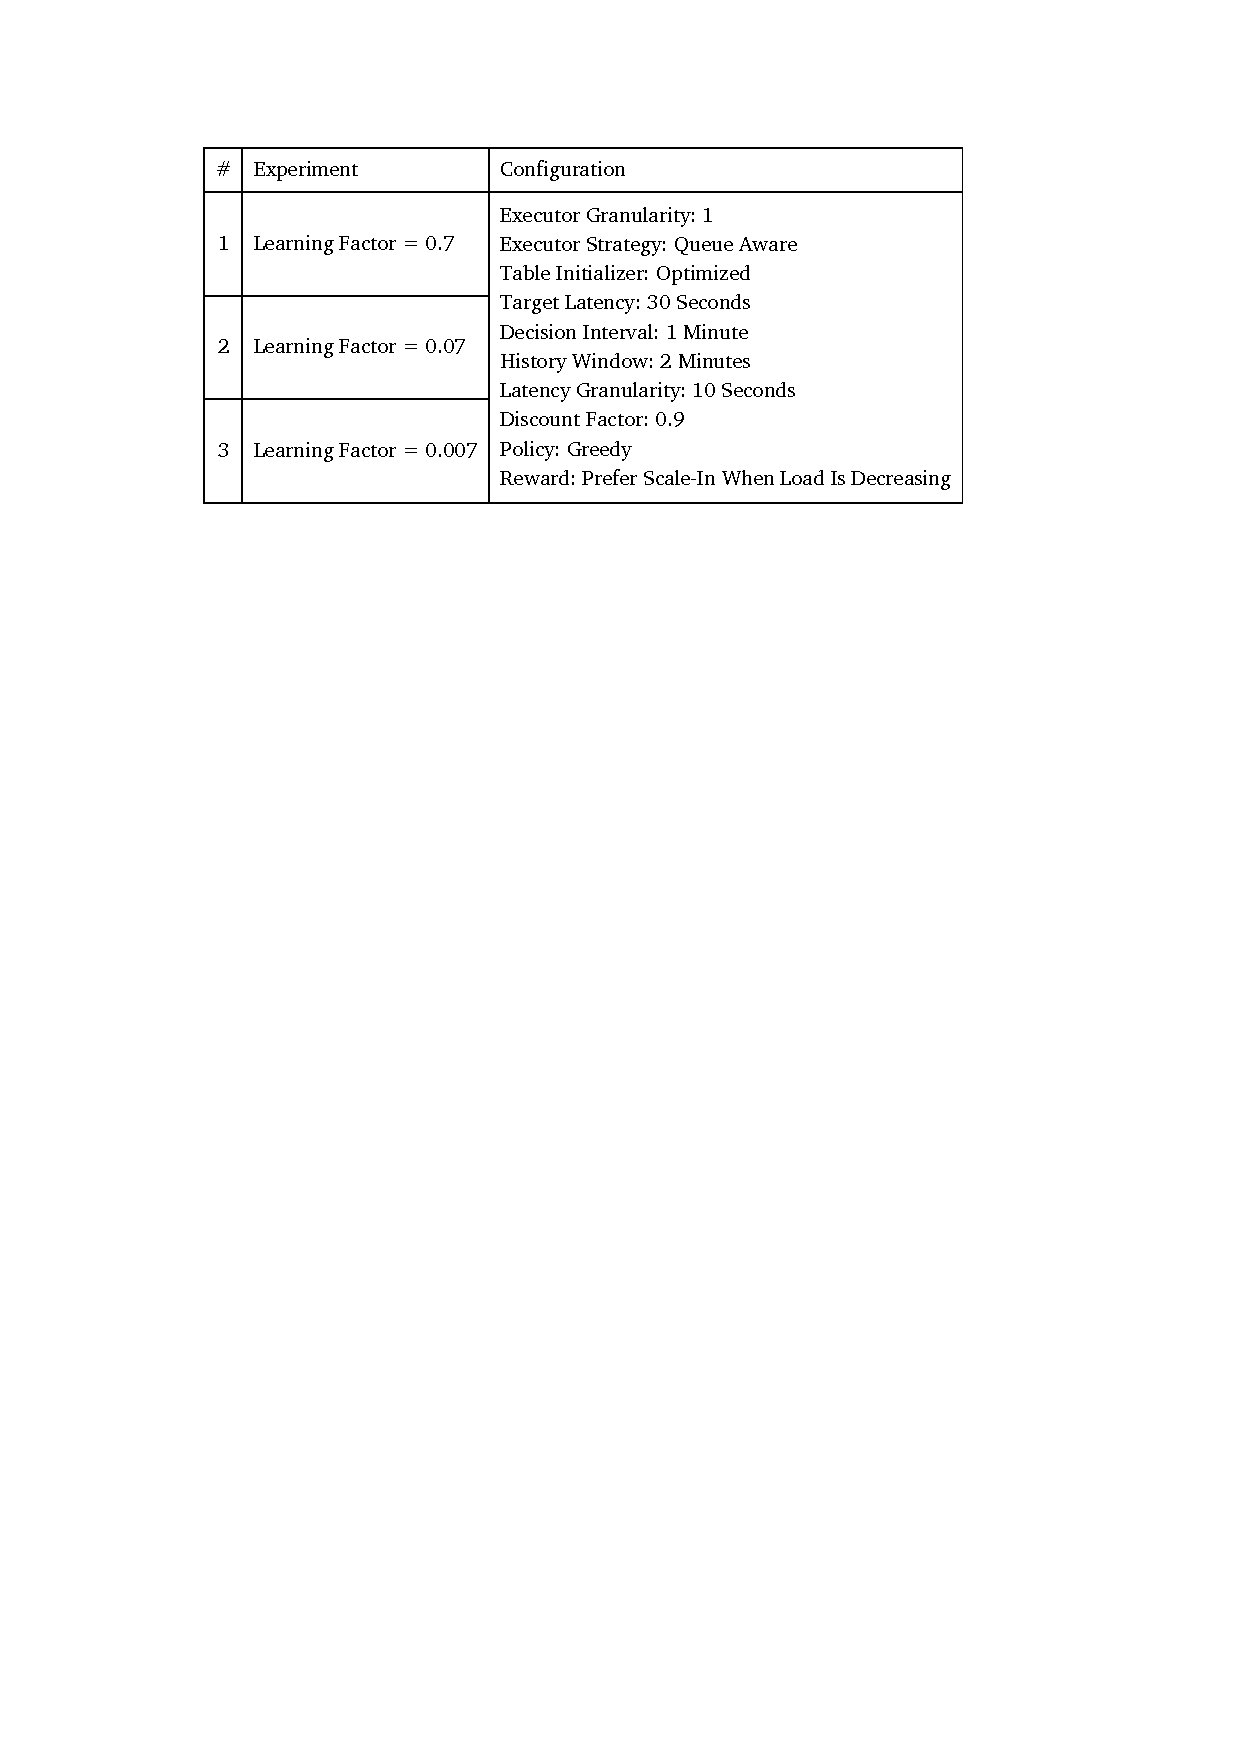
\includegraphics[clip,trim=3.3cm 21.18cm 4.5cm 2.5cm]{tables/ex5.pdf}
    \centering
    \caption{Learning Factor Configuration Parameters}
    \label{eval:tab:ex5}
\end{table}

Figure~\ref{eval:f:e5:w1:lat},~\ref{eval:f:e5:w1:exec},~\ref{eval:f:e5:w2:lat} and ~\ref{eval:f:e5:w2:exec} depicts detailed latency and executor charts for both workloads. Figure~\ref{eval:f:e5:w1:lat-c},~\ref{eval:f:e5:w1:exec-c},~\ref{eval:f:e5:w2:lat-c} and ~\ref{eval:f:e5:w2:exec-c} illustrates average and percentile charts for both workloads.

\begin{figure}[!htbp]
    \centering
    \begin{gnuplot}[terminal=epslatex, terminaloptions=color colortext]
        set terminal epslatex size 16cm,7.5cm
        set key inside center top horizontal box opaque
        set datafile separator ';'
        set xdata time
        set timefmt '%H:%M:%S'
        set xr ['0:00:00':'1:00:00']
        set yr [0:180]
        set xtics '00:00:00',600 nomirror
        set ytics 0,30 nomirror
        set y2r [0:180]
        set y2tics 0,30
        set samples 50000 
        unset mxtics
        unset mytics
        set grid ytics lc rgb "#bbbbbb" lw 1 lt 0
        set grid xtics lc rgb "#bbbbbb" lw 1 lt 0
        unset xl
        set yl 'Latency (Seconds)'
        plot 'ex/e5/w1/latency.csv' using 1:2 w l lc 'red' lw 4 smooth csplines t '0.7',\
        '' using 1:3 w l lc 'blue' lw 4 smooth csplines t '0.07',\
        '' using 1:4 w l lc 'black' lw 4 smooth csplines t '0.007'
    \end{gnuplot}
    \caption{Learning Factor -- W1 -- Latency}
    \label{eval:f:e5:w1:lat}
\end{figure}
\clearpage
\begin{figure}[H]
    \centering
    \begin{minipage}[h]{\linewidth}
        \centering
        \begin{gnuplot}[terminal=epslatex, terminaloptions=color colortext]
            set terminal epslatex size 16cm,7.5cm
            set key inside center top horizontal box opaque
            set datafile separator ';'
            set xdata time
            set timefmt '%H:%M:%S'
            set xr ['0:00:00':'1:00:00']
            set yr [2:28]
            set y2r [2:28]
            set ytics 0,4 nomirror
            set xtics '00:00:00',600 nomirror
            set y2tics 0,4
            unset mxtics
            unset mytics
            unset xl
            set grid ytics lc rgb "#bbbbbb" lw 1 lt 0
            set grid xtics lc rgb "#bbbbbb" lw 1 lt 0
            set yl 'Number of Executors'
            plot 'ex/e5/w1/exec.csv' using 1:2 w l lc 'red' lw 4 t '0.7',\
            '' using 1:3 w l lc 'blue' lw 4 t '0.07',\
            '' using 1:4 w l lc 'black' lw 4 t '0.007'
        \end{gnuplot}
        \caption{Learning Factor -- W1 -- Number of Executors}
        \label{eval:f:e5:w1:exec}
    \end{minipage}\hfil
    \begin{minipage}[h]{\linewidth}
        \centering
        \begin{gnuplot}[terminal=epslatex, terminaloptions=color colortext]
            set terminal epslatex size 16cm,7.5cm
            set key inside center top horizontal box opaque
            set datafile separator ';'
            set xdata time
            set timefmt '%H:%M:%S'
            set xr ['0:00:00':'1:00:00']
            set yr [0:130]
            set y2r [0:130]
            set xtics '00:00:00',600 nomirror
            set ytics 0,30 nomirror
            set y2tics 0,30
            unset mxtics
            unset mytics
            set samples 50000 
            unset xl
            set grid ytics lc rgb "#bbbbbb" lw 1 lt 0
            set grid xtics lc rgb "#bbbbbb" lw 1 lt 0
            set yl 'Latency (Seconds)'
            plot 'ex/e5/w2/latency.csv' using 1:2 w l lc 'red' lw 4 smooth csplines t '0.7',\
            '' using 1:3 w l lc 'blue' lw 4 smooth csplines t '0.07',\
            '' using 1:4 w l lc 'black' lw 4 smooth csplines t '0.007'
        \end{gnuplot}
        \caption{Learning Factor -- W2 -- Latency}
        \label{eval:f:e5:w2:lat}
    \end{minipage}\hfil
    \begin{minipage}[h]{\linewidth}
        \centering
        \begin{gnuplot}[terminal=epslatex, terminaloptions=color colortext]
            set terminal epslatex size 16cm,7.5cm
            set key inside center top horizontal box opaque
            set datafile separator ';'
            set xdata time
            set timefmt '%H:%M:%S'
            set xr ['0:00:00':'1:00:00']
            set yr [2:28]
            set y2r [2:28]
            set xtics '00:00:00',600 nomirror
            set ytics 0,4 nomirror
            set y2tics 0,4
            unset mxtics
            unset mytics
            unset xl
            set grid ytics lc rgb "#bbbbbb" lw 1 lt 0
            set grid xtics lc rgb "#bbbbbb" lw 1 lt 0
            set yl 'Number of Executors'
            plot 'ex/e5/w2/exec.csv' using 1:2 w l lc 'red' lw 4 t '0.7',\
            '' using 1:3 w l lc 'blue' lw 4 t '0.07',\
            '' using 1:4 w l lc 'black' lw 4 t '0.007'
        \end{gnuplot}
        \caption{Learning Factor -- W2 -- Number of Executors}
        \label{eval:f:e5:w2:exec}
    \end{minipage}
\end{figure}
\clearpage
\begin{figure}[H]
    \centering
    \begin{minipage}[h]{0.5\linewidth}
        \centering
        \begin{gnuplot}[terminal=epslatex, terminaloptions=color colortext]
            set terminal epslatex size 9cm,6cm
            set key inside center top horizontal box opaque
            set datafile separator ';'
            set xr [0.5:3.5]
            set yr [0:200]
            set ytics 0,30
            unset y2r
            unset y2tics
            set boxwidth 0.3 absolute
            set style fill empty
            unset xl
            set grid ytics lc rgb "#bbbbbb" lw 1 lt 0
            set grid xtics lc rgb "#bbbbbb" lw 1 lt 0
            set yl 'Latency (Seconds)'
            plot 'ex/e5/w1/latency-c.csv' using 1:2:3:4:5:xticlabels(7) with candlesticks lc 'black' lw 4 t 'Min/Max/Percentiles',\
            '' using 1:6:6:6:6 with linespoints pt 5 lc 'black' lw 4 t 'Average',\
            30 dashtype 2 lc 'black' lw 4 t 'Target'
        \end{gnuplot}
        \caption{Learning Factor -- W1 -- Latency}
        \label{eval:f:e5:w1:lat-c}
    \end{minipage}\hfil
    \begin{minipage}[h]{0.5\linewidth}
        \centering
        \begin{gnuplot}[terminal=epslatex, terminaloptions=color colortext]
            set terminal epslatex size 9cm,6cm
            set key inside center top horizontal box opaque
            set datafile separator ';'
            set xr [0.5:3.5]
            set yr [2:32]
            set ytics 0,4
            unset y2r
            unset y2tics
            set boxwidth 0.3 absolute
            set style fill empty
            unset xl
            set grid ytics lc rgb "#bbbbbb" lw 1 lt 0
            set grid xtics lc rgb "#bbbbbb" lw 1 lt 0
            set yl 'Number of Executors'
            plot 'ex/e5/w1/exec-c.csv' using 1:2:3:4:5:xticlabels(7) with candlesticks lc 'black' lw 4 t 'Min/Max/Percentiles',\
            '' using 1:6:6:6:6 with linespoints pt 5 lc 'black' lw 4 t 'Average' 
        \end{gnuplot}
        \caption{Learning Factor -- W1 -- Number of Executors}
        \label{eval:f:e5:w1:exec-c}
    \end{minipage}
    \begin{minipage}[h]{0.5\linewidth}
        \centering
        \begin{gnuplot}[terminal=epslatex, terminaloptions=color colortext]
            set terminal epslatex size 9cm,6cm
            set key inside center top horizontal box opaque
            set datafile separator ';'
            set xr [0.5:3.5]
            set yr [0:160]
            set ytics 0,30
            unset y2r
            unset y2tics
            set boxwidth 0.3 absolute
            set style fill empty
            unset xl
            set grid ytics lc rgb "#bbbbbb" lw 1 lt 0
            set grid xtics lc rgb "#bbbbbb" lw 1 lt 0
            set yl 'Latency (Seconds)'
            plot 'ex/e5/w2/latency-c.csv' using 1:2:3:4:5:xticlabels(7) with candlesticks lc 'black' lw 4 t 'Min/Max/Percentiles',\
            '' using 1:6:6:6:6 with linespoints pt 5 lc 'black' lw 4 t 'Average',\
            30 dashtype 2 lc 'black' lw 4 t 'Target'
        \end{gnuplot}
        \caption{Learning Factor -- W2 -- Latency}
        \label{eval:f:e5:w2:lat-c}
    \end{minipage}\hfil
    \begin{minipage}[h]{0.5\linewidth}
        \centering
        \begin{gnuplot}[terminal=epslatex, terminaloptions=color colortext]
            set terminal epslatex size 9cm,6cm
            set key inside center top horizontal box opaque
            set datafile separator ';'
            set xr [0.5:3.5]
            set yr [2:32]
            set ytics 0,4
            unset y2r
            unset y2tics
            set boxwidth 0.3 absolute
            set style fill empty
            unset xl
            set grid ytics lc rgb "#bbbbbb" lw 1 lt 0
            set grid xtics lc rgb "#bbbbbb" lw 1 lt 0
            set yl 'Number of Executors'
            plot 'ex/e5/w2/exec-c.csv' using 1:2:3:4:5:xticlabels(7) with candlesticks lc 'black' lw 4 t 'Min/Max/Percentiles','' using 1:6:6:6:6 with linespoints pt 5 lc 'black' lw 4 t 'Average' 
        \end{gnuplot}
        \caption{Learning Factor -- W2 -- Number of Executors}
        \label{eval:f:e5:w2:exec-c}
    \end{minipage}
\end{figure}
For Workload 1, learning factor of 0.7 achieves a better result both in terms of latency and number of executors. It is tempting to conclude that for unpredictable workloads, it is better to apply a higher learning factor.

But the above conclusion doesn't hold when we look at the result of Workload 2. In terms of latency, 0.007 is slightly below target latency which is better than 0.7 and 0.07. In terms of number of executors, it achieves an outstanding result of 8 executors on average. Combining latency and number of executors this is the best result that has been achieved for Workload 2.

It seems that the effect of learning factor is totally workload dependent and no generalized conclusion can be made based on these two workloads.
\clearpage
\section{Experiment 6: Discretization}
This experiment has been designed to evaluate the effect of discretization on Auto-Scaler's decisions. Discretization is applied to both latency and incoming messages. Table~\ref{eval:tab:ex6} describes the configuration parameters of this experiment.
\begin{table}[h]
    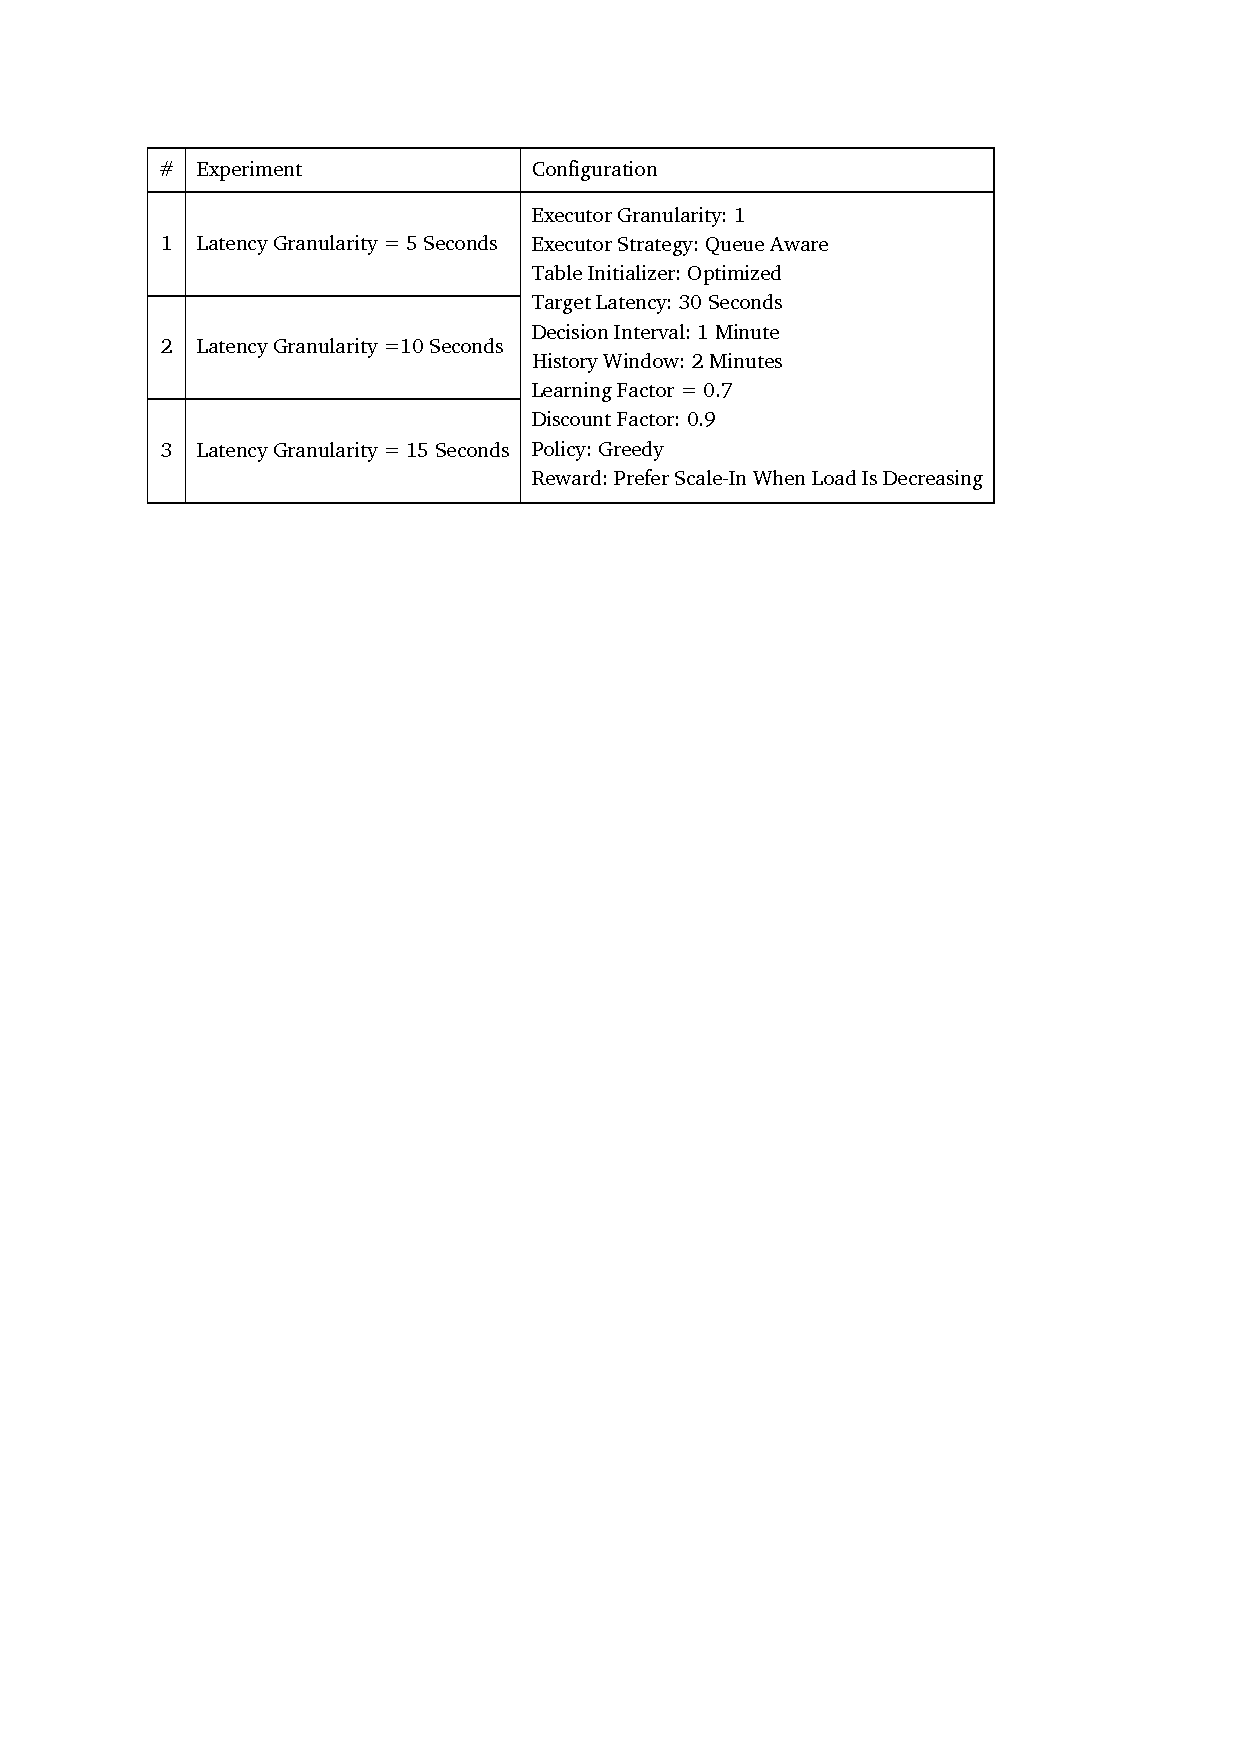
\includegraphics[clip,trim=2.2cm 21.18cm 3cm 2.5cm]{tables/ex6.pdf}
    \centering
    \caption{Discretization Configuration Parameters}
    \label{eval:tab:ex6}
\end{table}

Figure~\ref{eval:f:e6:w1:lat},~\ref{eval:f:e6:w1:exec},~\ref{eval:f:e6:w2:lat} and ~\ref{eval:f:e6:w2:exec} depicts detailed latency and executor charts for both workloads. Figure~\ref{eval:f:e6:w1:lat-c},~\ref{eval:f:e6:w1:exec-c},~\ref{eval:f:e6:w2:lat-c} and ~\ref{eval:f:e6:w2:exec-c} illustrates average and percentile charts for both workloads.

\begin{figure}[!htbp]
    \centering
    \begin{gnuplot}[terminal=epslatex, terminaloptions=color colortext]
        set terminal epslatex size 16cm,7.5cm
        set key inside center top horizontal box opaque
        set datafile separator ';'
        set xdata time
        set timefmt '%H:%M:%S'
        set xr ['0:00:00':'1:00:00']
        set yr [0:120]
        set xtics '00:00:00',600 nomirror
        set ytics 0,30 nomirror
        set y2r [0:120]
        set y2tics 0,30
        set samples 50000 
        unset mxtics
        unset mytics
        set grid ytics lc rgb "#bbbbbb" lw 1 lt 0
        set grid xtics lc rgb "#bbbbbb" lw 1 lt 0
        unset xl
        set yl 'Latency (Seconds)'
        plot 'ex/e6/w1/latency.csv' using 1:2 w l lc 'red' lw 4 smooth csplines t '5 Sec',\
        '' using 1:3 w l lc 'blue' lw 4 smooth csplines t '10 Sec',\
        '' using 1:4 w l lc 'black' lw 4 smooth csplines t '15 Sec'
    \end{gnuplot}
    \caption{Discretization -- W1 -- Latency}
    \label{eval:f:e6:w1:lat}
\end{figure}
\clearpage
\begin{figure}[H]
    \centering
    \begin{minipage}[h]{\linewidth}
        \centering
        \begin{gnuplot}[terminal=epslatex, terminaloptions=color colortext]
            set terminal epslatex size 16cm,7.5cm
            set key inside center top horizontal box opaque
            set datafile separator ';'
            set xdata time
            set timefmt '%H:%M:%S'
            set xr ['0:00:00':'1:00:00']
            set yr [2:28]
            set y2r [2:28]
            set ytics 0,4 nomirror
            set xtics '00:00:00',600 nomirror
            set y2tics 0,4
            unset mxtics
            unset mytics
            unset xl
            set grid ytics lc rgb "#bbbbbb" lw 1 lt 0
            set grid xtics lc rgb "#bbbbbb" lw 1 lt 0
            set yl 'Number of Executors'
            plot 'ex/e6/w1/exec.csv' using 1:2 w l lc 'red' lw 4 t '5 Sec',\
            '' using 1:3 w l lc 'blue' lw 4 t '10 Sec',\
            '' using 1:4 w l lc 'black' lw 4 t '15 Sec'
        \end{gnuplot}
        \caption{Discretization -- W1 -- Number of Executors}
        \label{eval:f:e6:w1:exec}
    \end{minipage}\hfil
    \begin{minipage}[h]{\linewidth}
        \centering
        \begin{gnuplot}[terminal=epslatex, terminaloptions=color colortext]
            set terminal epslatex size 16cm,7.5cm
            set key inside center top horizontal box opaque
            set datafile separator ';'
            set xdata time
            set timefmt '%H:%M:%S'
            set xr ['0:00:00':'1:00:00']
            set yr [0:130]
            set y2r [0:130]
            set xtics '00:00:00',600 nomirror
            set ytics 0,30 nomirror
            set y2tics 0,30
            unset mxtics
            unset mytics
            set samples 50000 
            unset xl
            set grid ytics lc rgb "#bbbbbb" lw 1 lt 0
            set grid xtics lc rgb "#bbbbbb" lw 1 lt 0
            set yl 'Latency (Seconds)'
            plot 'ex/e6/w2/latency.csv' using 1:2 w l lc 'red' lw 4 smooth csplines t '5 Sec',\
            '' using 1:3 w l lc 'blue' lw 4 smooth csplines t '10 Sec',\
            '' using 1:4 w l lc 'black' lw 4 smooth csplines t '15 Sec'
        \end{gnuplot}
        \caption{Discretization -- W2 -- Latency}
        \label{eval:f:e6:w2:lat}
    \end{minipage}\hfil
    \begin{minipage}[h]{\linewidth}
        \centering
        \begin{gnuplot}[terminal=epslatex, terminaloptions=color colortext]
            set terminal epslatex size 16cm,7.5cm
            set key inside center top horizontal box opaque
            set datafile separator ';'
            set xdata time
            set timefmt '%H:%M:%S'
            set xr ['0:00:00':'1:00:00']
            set yr [2:28]
            set y2r [2:28]
            set xtics '00:00:00',600 nomirror
            set ytics 0,4 nomirror
            set y2tics 0,4
            unset mxtics
            unset mytics
            unset xl
            set grid ytics lc rgb "#bbbbbb" lw 1 lt 0
            set grid xtics lc rgb "#bbbbbb" lw 1 lt 0
            set yl 'Number of Executors'
            plot 'ex/e6/w2/exec.csv' using 1:2 w l lc 'red' lw 4 t '5 Sec',\
            '' using 1:3 w l lc 'blue' lw 4 t '10 Sec',\
            '' using 1:4 w l lc 'black' lw 4 t '15 Sec'
        \end{gnuplot}
        \caption{Discretization -- W2 -- Number of Executors}
        \label{eval:f:e6:w2:exec}
    \end{minipage}
\end{figure}
\clearpage
\begin{figure}[H]
    \centering
    \begin{minipage}[h]{0.5\linewidth}
        \centering
        \begin{gnuplot}[terminal=epslatex, terminaloptions=color colortext]
            set terminal epslatex size 9cm,6cm
            set key inside center top horizontal box opaque
            set datafile separator ';'
            set xr [0.5:3.5]
            set yr [0:160]
            set ytics 0,30
            unset y2r
            unset y2tics
            set boxwidth 0.3 absolute
            set style fill empty
            unset xl
            set grid ytics lc rgb "#bbbbbb" lw 1 lt 0
            set grid xtics lc rgb "#bbbbbb" lw 1 lt 0
            set yl 'Latency (Seconds)'
            plot 'ex/e6/w1/latency-c.csv' using 1:2:3:4:5:xticlabels(7) with candlesticks lc 'black' lw 4 t 'Min/Max/Percentiles',\
            '' using 1:6:6:6:6 with linespoints pt 5 lc 'black' lw 4 t 'Average',\
            30 dashtype 2 lc 'black' lw 4 t 'Target'
        \end{gnuplot}
        \caption{Discretization -- W1 -- Latency}
        \label{eval:f:e6:w1:lat-c}
    \end{minipage}\hfil
    \begin{minipage}[h]{0.5\linewidth}
        \centering
        \begin{gnuplot}[terminal=epslatex, terminaloptions=color colortext]
            set terminal epslatex size 9cm,6cm
            set key inside center top horizontal box opaque
            set datafile separator ';'
            set xr [0.5:3.5]
            set yr [2:32]
            set ytics 0,4
            unset y2r
            unset y2tics
            set boxwidth 0.3 absolute
            set style fill empty
            unset xl
            set grid ytics lc rgb "#bbbbbb" lw 1 lt 0
            set grid xtics lc rgb "#bbbbbb" lw 1 lt 0
            set yl 'Number of Executors'
            plot 'ex/e6/w1/exec-c.csv' using 1:2:3:4:5:xticlabels(7) with candlesticks lc 'black' lw 4 t 'Min/Max/Percentiles',\
            '' using 1:6:6:6:6 with linespoints pt 5 lc 'black' lw 4 t 'Average' 
        \end{gnuplot}
        \caption{Discretization -- W1 -- Number of Executors}
        \label{eval:f:e6:w1:exec-c}
    \end{minipage}
    \begin{minipage}[h]{0.5\linewidth}
        \centering
        \begin{gnuplot}[terminal=epslatex, terminaloptions=color colortext]
            set terminal epslatex size 9cm,6cm
            set key inside center top horizontal box opaque
            set datafile separator ';'
            set xr [0.5:3.5]
            set yr [0:160]
            set ytics 0,30
            unset y2r
            unset y2tics
            set boxwidth 0.3 absolute
            set style fill empty
            unset xl
            set grid ytics lc rgb "#bbbbbb" lw 1 lt 0
            set grid xtics lc rgb "#bbbbbb" lw 1 lt 0
            set yl 'Latency (Seconds)'
            plot 'ex/e6/w2/latency-c.csv' using 1:2:3:4:5:xticlabels(7) with candlesticks lc 'black' lw 4 t 'Min/Max/Percentiles',\
            '' using 1:6:6:6:6 with linespoints pt 5 lc 'black' lw 4 t 'Average',\
            30 dashtype 2 lc 'black' lw 4 t 'Target'
        \end{gnuplot}
        \caption{Discretization -- W2 -- Latency}
        \label{eval:f:e6:w2:lat-c}
    \end{minipage}\hfil
    \begin{minipage}[h]{0.5\linewidth}
        \centering
        \begin{gnuplot}[terminal=epslatex, terminaloptions=color colortext]
            set terminal epslatex size 9cm,6cm
            set key inside center top horizontal box opaque
            set datafile separator ';'
            set xr [0.5:3.5]
            set yr [2:32]
            set ytics 0,4
            unset y2r
            unset y2tics
            set boxwidth 0.3 absolute
            set style fill empty
            unset xl
            set grid ytics lc rgb "#bbbbbb" lw 1 lt 0
            set grid xtics lc rgb "#bbbbbb" lw 1 lt 0
            set yl 'Number of Executors'
            plot 'ex/e6/w2/exec-c.csv' using 1:2:3:4:5:xticlabels(7) with candlesticks lc 'black' lw 4 t 'Min/Max/Percentiles','' using 1:6:6:6:6 with linespoints pt 5 lc 'black' lw 4 t 'Average' 
        \end{gnuplot}
        \caption{Discretization -- W2 -- Number of Executors}
        \label{eval:f:e6:w2:exec-c}
    \end{minipage}
\end{figure}

Similar to learning factor, discretization seems to be workload dependent and no generalized conclusion can be made.

\clearpage
\section{Experiment 7: Value Iteration}
\textcite{dutreilh:hal-01122123} claimed that Value Iteration algorithm helps to initialize the state table and speedup learning process. Authors conducted an experiment which was based on a sinusoidal workload. Agent is trained in first period of rotation and then standard Q-Learning is used for next rounds. However, training based on sinusoidal workload is not so challenging. In this experiment the agent is trained using a different data set than the actual workload. State space is initialized after 5, 10 and 20 minutes of training period and then Auto-Scaler's behavior is evaluated under both workloads. During training \lstinline|decreasingOneMinusEpsilon| policy is used to help agent discover the environment. However, during the evaluation greedy policy is used. Table~\ref{eval:tab:ex7} describes the configuration parameters of this experiment.
\begin{table}[h]
    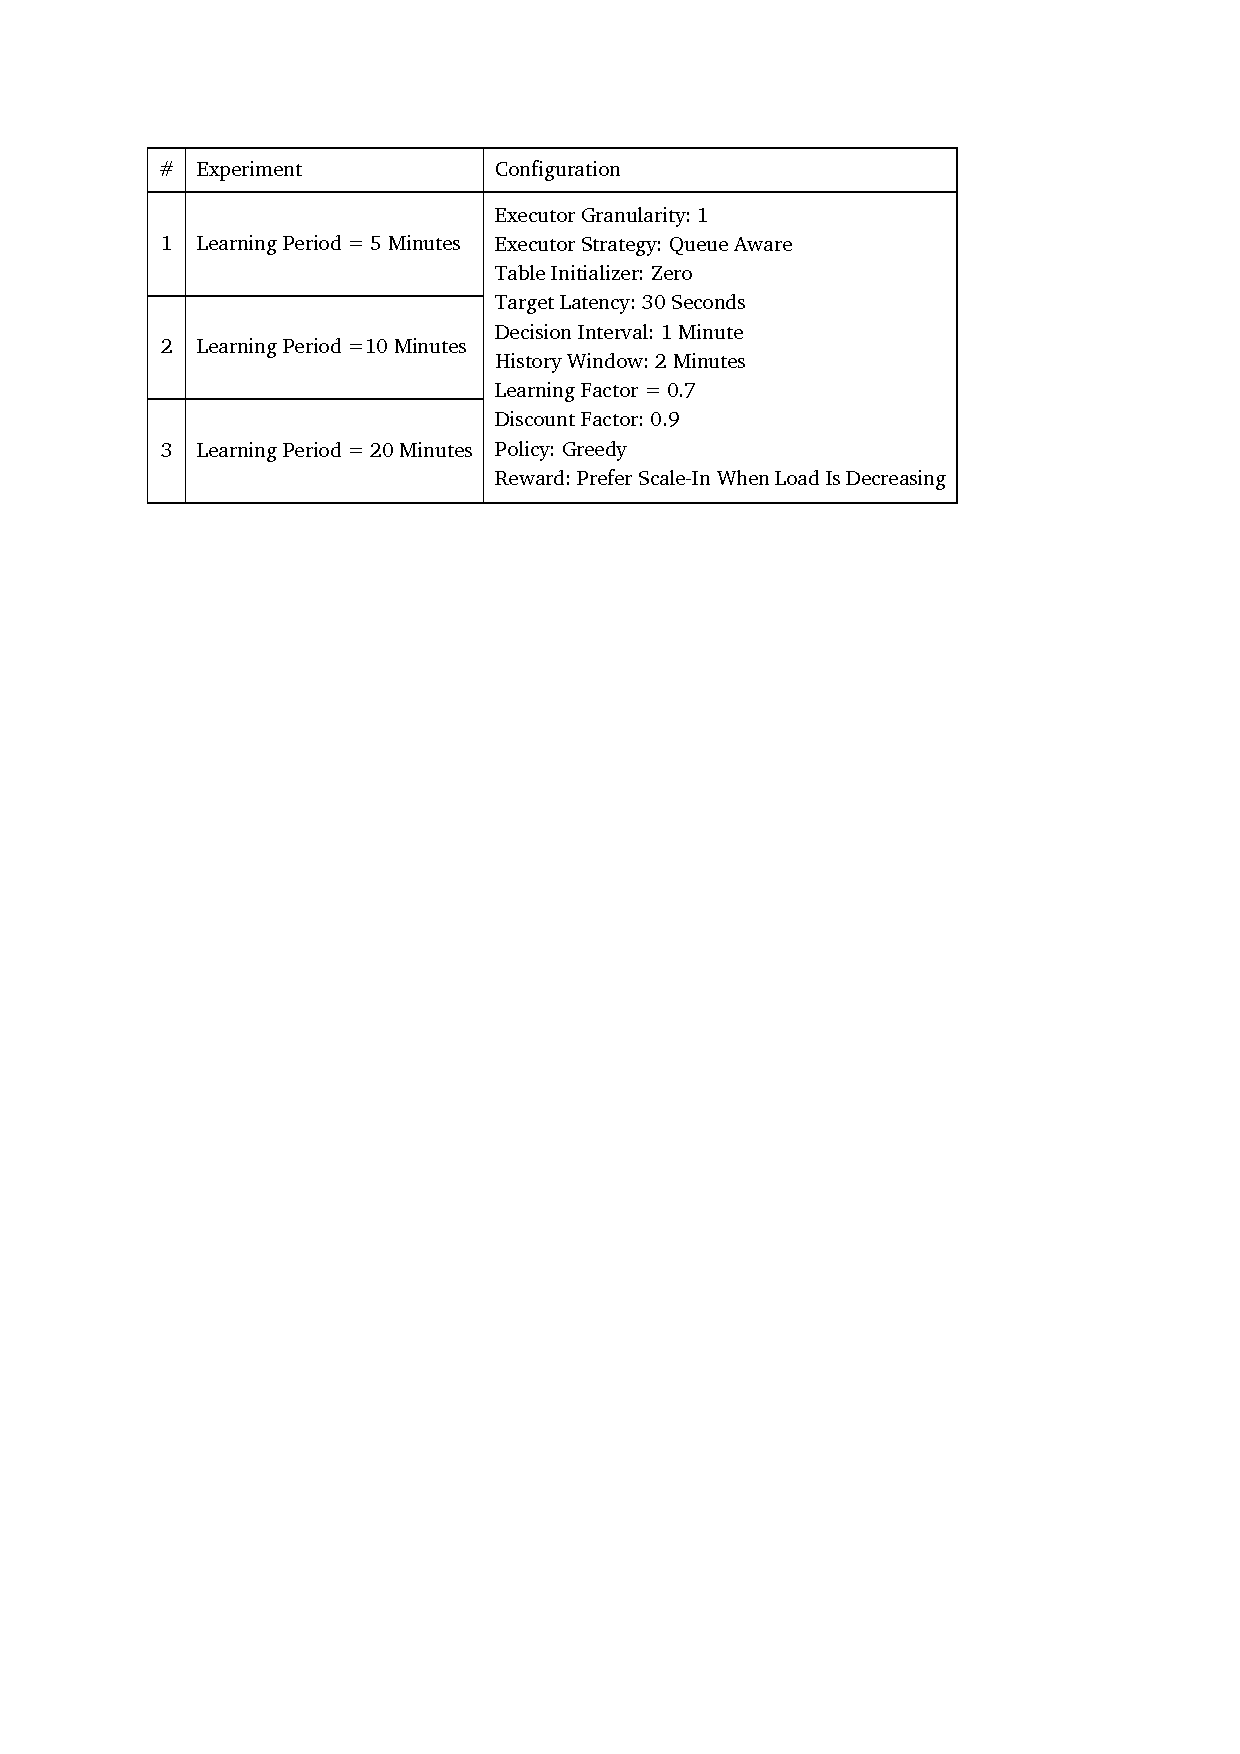
\includegraphics[clip,trim=2.4cm 21.18cm 4.65cm 2.5cm]{tables/ex7.pdf}
    \centering
    \caption{Value Iteration Configuration Parameters}
    \label{eval:tab:ex7}
\end{table}

Figure~\ref{eval:f:e7:w1:lat},~\ref{eval:f:e7:w1:exec},~\ref{eval:f:e7:w2:lat} and ~\ref{eval:f:e7:w2:exec} depicts detailed latency and executor charts for both workloads. Figure~\ref{eval:f:e7:w1:lat-c},~\ref{eval:f:e7:w1:exec-c},~\ref{eval:f:e7:w2:lat-c} and ~\ref{eval:f:e7:w2:exec-c} illustrates average and percentile charts for both workloads.

\begin{figure}[!htbp]
    \centering
    \begin{gnuplot}[terminal=epslatex, terminaloptions=color colortext]
        set terminal epslatex size 16cm,7.5cm
        set key inside center top horizontal box opaque
        set datafile separator ';'
        set xdata time
        set timefmt '%H:%M:%S'
        set xr ['0:00:00':'1:00:00']
        set yr [0:220]
        set xtics '00:00:00',600 nomirror
        set ytics 0,30 nomirror
        set y2r [0:220]
        set y2tics 0,30
        set samples 50000 
        unset mxtics
        unset mytics
        set grid ytics lc rgb "#bbbbbb" lw 1 lt 0
        set grid xtics lc rgb "#bbbbbb" lw 1 lt 0
        unset xl
        set yl 'Latency (Seconds)'
        plot 'ex/e7/w1/latency.csv' using 1:2 w l lc 'red' lw 4 smooth csplines t '5 Min',\
        '' using 1:3 w l lc 'blue' lw 4 smooth csplines t '10 Min',\
        '' using 1:4 w l lc 'black' lw 4 smooth csplines t '20 Min'
    \end{gnuplot}
    \caption{Value Iteration -- W1 -- Latency}
    \label{eval:f:e7:w1:lat}
\end{figure}
\clearpage
\begin{figure}[H]
    \centering
    \begin{minipage}[h]{\linewidth}
        \centering
        \begin{gnuplot}[terminal=epslatex, terminaloptions=color colortext]
            set terminal epslatex size 16cm,7.5cm
            set key inside center top horizontal box opaque
            set datafile separator ';'
            set xdata time
            set timefmt '%H:%M:%S'
            set xr ['0:00:00':'1:00:00']
            set yr [2:28]
            set y2r [2:28]
            set ytics 0,4 nomirror
            set xtics '00:00:00',600 nomirror
            set y2tics 0,4
            unset mxtics
            unset mytics
            unset xl
            set grid ytics lc rgb "#bbbbbb" lw 1 lt 0
            set grid xtics lc rgb "#bbbbbb" lw 1 lt 0
            set yl 'Number of Executors'
            plot 'ex/e7/w1/exec.csv' using 1:2 w l lc 'red' lw 4 t '5 Min',\
            '' using 1:3 w l lc 'blue' lw 4 t '10 Min',\
            '' using 1:4 w l lc 'black' lw 4 t '20 Min'
        \end{gnuplot}
        \caption{Value Iteration -- W1 -- Number of Executors}
        \label{eval:f:e7:w1:exec}
    \end{minipage}\hfil
    \begin{minipage}[h]{\linewidth}
        \centering
        \begin{gnuplot}[terminal=epslatex, terminaloptions=color colortext]
            set terminal epslatex size 16cm,7.5cm
            set key inside center top horizontal box opaque
            set datafile separator ';'
            set xdata time
            set timefmt '%H:%M:%S'
            set xr ['0:00:00':'1:00:00']
            set yr [0:160]
            set y2r [0:160]
            set xtics '00:00:00',600 nomirror
            set ytics 0,30 nomirror
            set y2tics 0,30
            unset mxtics
            unset mytics
            set samples 50000 
            unset xl
            set grid ytics lc rgb "#bbbbbb" lw 1 lt 0
            set grid xtics lc rgb "#bbbbbb" lw 1 lt 0
            set yl 'Latency (Seconds)'
            plot 'ex/e7/w2/latency.csv' using 1:2 w l lc 'red' lw 4 smooth csplines t '5 Min',\
            '' using 1:3 w l lc 'blue' lw 4 smooth csplines t '10 Min',\
            '' using 1:4 w l lc 'black' lw 4 smooth csplines t '20 Min'
        \end{gnuplot}
        \caption{Value Iteration -- W2 -- Latency}
        \label{eval:f:e7:w2:lat}
    \end{minipage}\hfil
    \begin{minipage}[h]{\linewidth}
        \centering
        \begin{gnuplot}[terminal=epslatex, terminaloptions=color colortext]
            set terminal epslatex size 16cm,7.5cm
            set key inside center top horizontal box opaque
            set datafile separator ';'
            set xdata time
            set timefmt '%H:%M:%S'
            set xr ['0:00:00':'1:00:00']
            set yr [2:28]
            set y2r [2:28]
            set xtics '00:00:00',600 nomirror
            set ytics 0,4 nomirror
            set y2tics 0,4
            unset mxtics
            unset mytics
            unset xl
            set grid ytics lc rgb "#bbbbbb" lw 1 lt 0
            set grid xtics lc rgb "#bbbbbb" lw 1 lt 0
            set yl 'Number of Executors'
            plot 'ex/e7/w2/exec.csv' using 1:2 w l lc 'red' lw 4 t '5 Min',\
            '' using 1:3 w l lc 'blue' lw 4 t '10 Min',\
            '' using 1:4 w l lc 'black' lw 4 t '20 Min'
        \end{gnuplot}
        \caption{Value Iteration -- W2 -- Number of Executors}
        \label{eval:f:e7:w2:exec}
    \end{minipage}
\end{figure}
\clearpage
\begin{figure}[H]
    \centering
    \begin{minipage}[h]{0.5\linewidth}
        \centering
        \begin{gnuplot}[terminal=epslatex, terminaloptions=color colortext]
            set terminal epslatex size 9cm,6cm
            set key inside center top horizontal box opaque
            set datafile separator ';'
            set xr [0.5:3.5]
            set yr [0:280]
            set ytics 0,30
            unset y2r
            unset y2tics
            set boxwidth 0.3 absolute
            set style fill empty
            unset xl
            set grid ytics lc rgb "#bbbbbb" lw 1 lt 0
            set grid xtics lc rgb "#bbbbbb" lw 1 lt 0
            set yl 'Latency (Seconds)'
            plot 'ex/e7/w1/latency-c.csv' using 1:2:3:4:5:xticlabels(7) with candlesticks lc 'black' lw 4 t 'Min/Max/Percentiles',\
            '' using 1:6:6:6:6 with linespoints pt 5 lc 'black' lw 4 t 'Average',\
            30 dashtype 2 lc 'black' lw 4 t 'Target'
        \end{gnuplot}
        \caption{Value Iteration -- W1 -- Latency}
        \label{eval:f:e7:w1:lat-c}
    \end{minipage}\hfil
    \begin{minipage}[h]{0.5\linewidth}
        \centering
        \begin{gnuplot}[terminal=epslatex, terminaloptions=color colortext]
            set terminal epslatex size 9cm,6cm
            set key inside center top horizontal box opaque
            set datafile separator ';'
            set xr [0.5:3.5]
            set yr [2:32]
            set ytics 0,4
            unset y2r
            unset y2tics
            set boxwidth 0.3 absolute
            set style fill empty
            unset xl
            set grid ytics lc rgb "#bbbbbb" lw 1 lt 0
            set grid xtics lc rgb "#bbbbbb" lw 1 lt 0
            set yl 'Number of Executors'
            plot 'ex/e7/w1/exec-c.csv' using 1:2:3:4:5:xticlabels(7) with candlesticks lc 'black' lw 4 t 'Min/Max/Percentiles',\
            '' using 1:6:6:6:6 with linespoints pt 5 lc 'black' lw 4 t 'Average' 
        \end{gnuplot}
        \caption{Value Iteration -- W1 -- Number of Executors}
        \label{eval:f:e7:w1:exec-c}
    \end{minipage}
    \begin{minipage}[h]{0.5\linewidth}
        \centering
        \begin{gnuplot}[terminal=epslatex, terminaloptions=color colortext]
            set terminal epslatex size 9cm,6cm
            set key inside center top horizontal box opaque
            set datafile separator ';'
            set xr [0.5:3.5]
            set yr [0:200]
            set ytics 0,30
            unset y2r
            unset y2tics
            set boxwidth 0.3 absolute
            set style fill empty
            unset xl
            set grid ytics lc rgb "#bbbbbb" lw 1 lt 0
            set grid xtics lc rgb "#bbbbbb" lw 1 lt 0
            set yl 'Latency (Seconds)'
            plot 'ex/e7/w2/latency-c.csv' using 1:2:3:4:5:xticlabels(7) with candlesticks lc 'black' lw 4 t 'Min/Max/Percentiles',\
            '' using 1:6:6:6:6 with linespoints pt 5 lc 'black' lw 4 t 'Average',\
            30 dashtype 2 lc 'black' lw 4 t 'Target'
        \end{gnuplot}
        \caption{Value Iteration -- W2 -- Latency}
        \label{eval:f:e7:w2:lat-c}
    \end{minipage}\hfil
    \begin{minipage}[h]{0.5\linewidth}
        \centering
        \begin{gnuplot}[terminal=epslatex, terminaloptions=color colortext]
            set terminal epslatex size 9cm,6cm
            set key inside center top horizontal box opaque
            set datafile separator ';'
            set xr [0.5:3.5]
            set yr [2:32]
            set ytics 0,4
            unset y2r
            unset y2tics
            set boxwidth 0.3 absolute
            set style fill empty
            unset xl
            set grid ytics lc rgb "#bbbbbb" lw 1 lt 0
            set grid xtics lc rgb "#bbbbbb" lw 1 lt 0
            set yl 'Number of Executors'
            plot 'ex/e7/w2/exec-c.csv' using 1:2:3:4:5:xticlabels(7) with candlesticks lc 'black' lw 4 t 'Min/Max/Percentiles','' using 1:6:6:6:6 with linespoints pt 5 lc 'black' lw 4 t 'Average' 
        \end{gnuplot}
        \caption{Value Iteration -- W2 -- Number of Executors}
        \label{eval:f:e7:w2:exec-c}
    \end{minipage}
\end{figure}

Looking at the results and combining them with the results of \textcite{dutreilh:hal-01122123} reveals a couple of interesting points.
\begin{itemize}
    \item If the sample data set is a good representative of actual workload, then Value Iteration is quite useful.
    \item \emph{The more training, the better outcome} does not hold for streaming workloads. Since it is possible to introduce wrong information into state space at any time. As can be seen from this experiment, ten minute training was worse than five minute training.
\end{itemize}
The major question that arises is \emph{what is the optimal period of training?} Since the workload is changing in an unpredictable manner, finding a near optimal learning period is extremely difficult and workload dependent.
\clearpage
\section{Experiment 8: Hitting Target}
So far we have experimented the behavior of Auto-Scaler under different configurations. However, target latency has been set to 30 seconds in all experiments. In this experiment, we will set other target values to evaluate whether Q-Learning approach is able to hit multiple targets. Table~\ref{eval:tab:ex8} describes the configuration parameters of this experiment. Note that different sliding windows are used for Workload 1 and Workload 2. Three minute history window performs better for Workload 1, so this option is adopted. Additionally, based on previous experiments, setting target value to more than 30 seconds makes it too easy for Auto-Scaler. Thus, those cases are not tested. 
\begin{table}[h]
    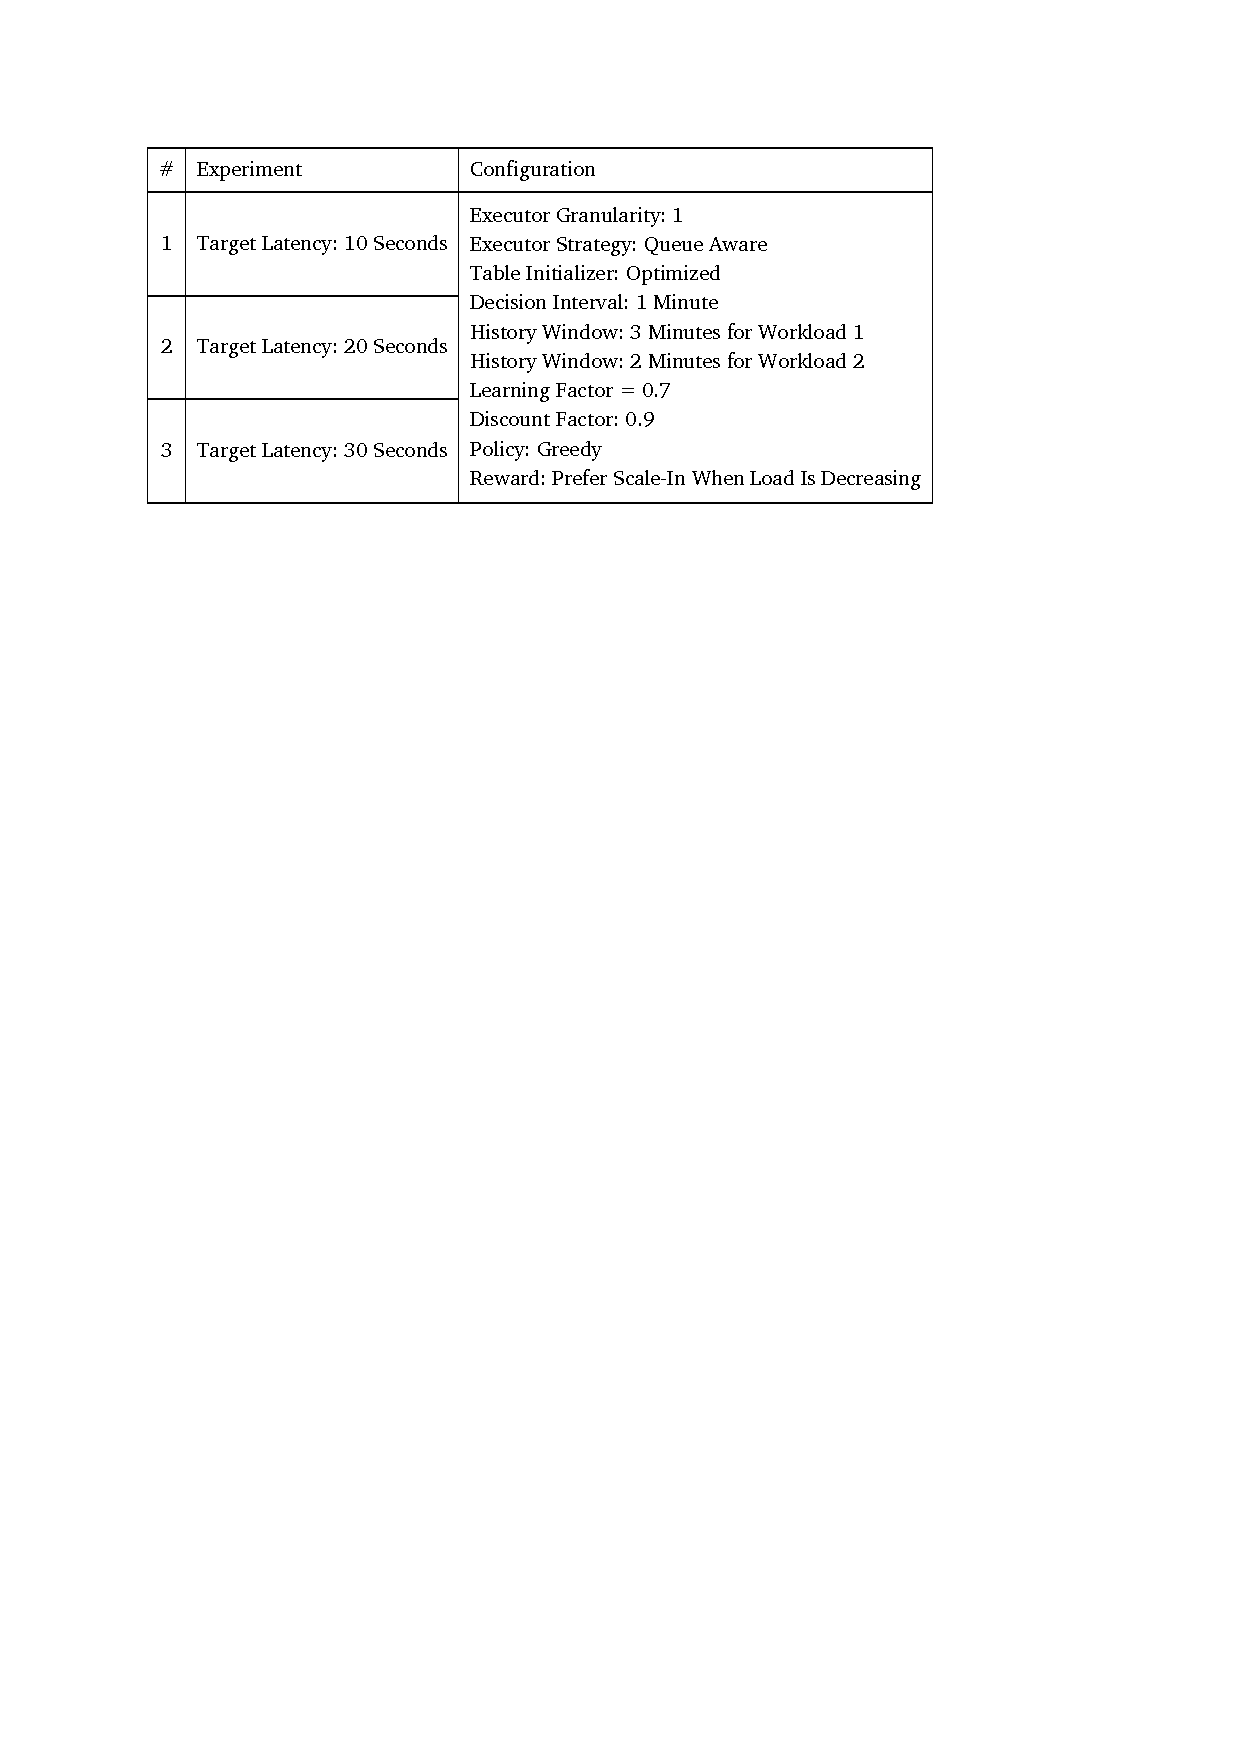
\includegraphics[clip,trim=2.4cm 21.18cm 5.1cm 2.5cm]{tables/ex8.pdf}
    \centering
    \caption{Hitting Target Configuration Parameters}
    \label{eval:tab:ex8}
\end{table}

Figure~\ref{eval:f:e8:w1:lat},~\ref{eval:f:e8:w1:exec},~\ref{eval:f:e8:w2:lat} and ~\ref{eval:f:e8:w2:exec} depicts detailed latency and executor charts for both workloads. Figure~\ref{eval:f:e8:w1:lat-c},~\ref{eval:f:e8:w1:exec-c},~\ref{eval:f:e8:w2:lat-c} and ~\ref{eval:f:e8:w2:exec-c} illustrates average and percentile charts for both workloads.

\begin{figure}[!htbp]
    \centering
    \begin{gnuplot}[terminal=epslatex, terminaloptions=color colortext]
        set terminal epslatex size 16cm,7.5cm
        set key inside center top horizontal box opaque
        set datafile separator ';'
        set xdata time
        set timefmt '%H:%M:%S'
        set xr ['0:00:00':'1:00:00']
        set yr [0:120]
        set xtics '00:00:00',600 nomirror
        set ytics 0,30 nomirror
        set y2r [0:120]
        set y2tics 0,30
        set samples 50000 
        unset mxtics
        unset mytics
        set grid ytics lc rgb "#bbbbbb" lw 1 lt 0
        set grid xtics lc rgb "#bbbbbb" lw 1 lt 0
        unset xl
        set yl 'Latency (Seconds)'
        plot 'ex/e8/w1/latency.csv' using 1:2 w l lc 'red' lw 4 smooth csplines t '10 Sec',\
        '' using 1:3 w l lc 'blue' lw 4 smooth csplines t '20 Sec',\
        '' using 1:4 w l lc 'black' lw 4 smooth csplines t '30 Sec'
    \end{gnuplot}
    \caption{Hitting Target -- W1 -- Latency}
    \label{eval:f:e8:w1:lat}
\end{figure}
\clearpage
\begin{figure}[H]
    \centering
    \begin{minipage}[h]{\linewidth}
        \centering
        \begin{gnuplot}[terminal=epslatex, terminaloptions=color colortext]
            set terminal epslatex size 16cm,7.5cm
            set key inside center top horizontal box opaque
            set datafile separator ';'
            set xdata time
            set timefmt '%H:%M:%S'
            set xr ['0:00:00':'1:00:00']
            set yr [2:28]
            set y2r [2:28]
            set ytics 0,4 nomirror
            set xtics '00:00:00',600 nomirror
            set y2tics 0,4
            unset mxtics
            unset mytics
            unset xl
            set grid ytics lc rgb "#bbbbbb" lw 1 lt 0
            set grid xtics lc rgb "#bbbbbb" lw 1 lt 0
            set yl 'Number of Executors'
            plot 'ex/e8/w1/exec.csv' using 1:2 w l lc 'red' lw 4 t '10 Sec',\
            '' using 1:3 w l lc 'blue' lw 4 t '20 Sec',\
            '' using 1:4 w l lc 'black' lw 4 t '30 Sec'
        \end{gnuplot}
        \caption{Hitting Target -- W1 -- Number of Executors}
        \label{eval:f:e8:w1:exec}
    \end{minipage}\hfil
    \begin{minipage}[h]{\linewidth}
        \centering
        \begin{gnuplot}[terminal=epslatex, terminaloptions=color colortext]
            set terminal epslatex size 16cm,7.5cm
            set key inside center top horizontal box opaque
            set datafile separator ';'
            set xdata time
            set timefmt '%H:%M:%S'
            set xr ['0:00:00':'1:00:00']
            set yr [0:120]
            set y2r [0:120]
            set xtics '00:00:00',600 nomirror
            set ytics 0,30 nomirror
            set y2tics 0,30
            unset mxtics
            unset mytics
            set samples 50000 
            unset xl
            set grid ytics lc rgb "#bbbbbb" lw 1 lt 0
            set grid xtics lc rgb "#bbbbbb" lw 1 lt 0
            set yl 'Latency (Seconds)'
            plot 'ex/e8/w2/latency.csv' using 1:2 w l lc 'red' lw 4 smooth csplines t '10 Sec',\
            '' using 1:3 w l lc 'blue' lw 4 smooth csplines t '20 Sec',\
            '' using 1:4 w l lc 'black' lw 4 smooth csplines t '30 Sec'
        \end{gnuplot}
        \caption{Hitting Target -- W2 -- Latency}
        \label{eval:f:e8:w2:lat}
    \end{minipage}\hfil
    \begin{minipage}[h]{\linewidth}
        \centering
        \begin{gnuplot}[terminal=epslatex, terminaloptions=color colortext]
            set terminal epslatex size 16cm,7.5cm
            set key inside center top horizontal box opaque
            set datafile separator ';'
            set xdata time
            set timefmt '%H:%M:%S'
            set xr ['0:00:00':'1:00:00']
            set yr [2:28]
            set y2r [2:28]
            set xtics '00:00:00',600 nomirror
            set ytics 0,4 nomirror
            set y2tics 0,4
            unset mxtics
            unset mytics
            unset xl
            set grid ytics lc rgb "#bbbbbb" lw 1 lt 0
            set grid xtics lc rgb "#bbbbbb" lw 1 lt 0
            set yl 'Number of Executors'
            plot 'ex/e8/w2/exec.csv' using 1:2 w l lc 'red' lw 4 t '10 Sec',\
            '' using 1:3 w l lc 'blue' lw 4 t '20 Sec',\
            '' using 1:4 w l lc 'black' lw 4 t '30 Sec'
        \end{gnuplot}
        \caption{Hitting Target -- W2 -- Number of Executors}
        \label{eval:f:e8:w2:exec}
    \end{minipage}
\end{figure}
\clearpage
\begin{figure}[H]
    \centering
    \begin{minipage}[h]{0.5\linewidth}
        \centering
        \begin{gnuplot}[terminal=epslatex, terminaloptions=color colortext]
            set terminal epslatex size 9cm,6cm
            set key inside center top horizontal box opaque
            set datafile separator ';'
            set xr [0.5:3.5]
            set yr [0:120]
            set ytics 0,20
            unset y2r
            unset y2tics
            set boxwidth 0.3 absolute
            set style fill empty
            unset xl
            set grid ytics lc rgb "#bbbbbb" lw 1 lt 0
            set grid xtics lc rgb "#bbbbbb" lw 1 lt 0
            set yl 'Latency (Seconds)'
            plot 'ex/e8/w1/latency-c.csv' using 1:2:3:4:5:xticlabels(7) with candlesticks lc 'black' lw 4 t 'Min/Max/Percentiles',\
            '' using 1:6:6:6:6 with linespoints pt 5 lc 'black' lw 4 t 'Average'
        \end{gnuplot}
        \caption{Hitting Target -- W1 -- Latency}
        \label{eval:f:e8:w1:lat-c}
    \end{minipage}\hfil
    \begin{minipage}[h]{0.5\linewidth}
        \centering
        \begin{gnuplot}[terminal=epslatex, terminaloptions=color colortext]
            set terminal epslatex size 9cm,6cm
            set key inside center top horizontal box opaque
            set datafile separator ';'
            set xr [0.5:3.5]
            set yr [2:32]
            set ytics 0,4
            unset y2r
            unset y2tics
            set boxwidth 0.3 absolute
            set style fill empty
            unset xl
            set grid ytics lc rgb "#bbbbbb" lw 1 lt 0
            set grid xtics lc rgb "#bbbbbb" lw 1 lt 0
            set yl 'Number of Executors'
            plot 'ex/e8/w1/exec-c.csv' using 1:2:3:4:5:xticlabels(7) with candlesticks lc 'black' lw 4 t 'Min/Max/Percentiles',\
            '' using 1:6:6:6:6 with linespoints pt 5 lc 'black' lw 4 t 'Average' 
        \end{gnuplot}
        \caption{Hitting Target -- W1 -- Number of Executors}
        \label{eval:f:e8:w1:exec-c}
    \end{minipage}
    \begin{minipage}[h]{0.5\linewidth}
        \centering
        \begin{gnuplot}[terminal=epslatex, terminaloptions=color colortext]
            set terminal epslatex size 9cm,6cm
            set key inside center top horizontal box opaque
            set datafile separator ';'
            set xr [0.5:3.5]
            set yr [0:140]
            set ytics 0,20
            unset y2r
            unset y2tics
            set boxwidth 0.3 absolute
            set style fill empty
            unset xl
            set grid ytics lc rgb "#bbbbbb" lw 1 lt 0
            set grid xtics lc rgb "#bbbbbb" lw 1 lt 0
            set yl 'Latency (Seconds)'
            plot 'ex/e8/w2/latency-c.csv' using 1:2:3:4:5:xticlabels(7) with candlesticks lc 'black' lw 4 t 'Min/Max/Percentiles',\
            '' using 1:6:6:6:6 with linespoints pt 5 lc 'black' lw 4 t 'Average'
        \end{gnuplot}
        \caption{Hitting Target -- W2 -- Latency}
        \label{eval:f:e8:w2:lat-c}
    \end{minipage}\hfil
    \begin{minipage}[h]{0.5\linewidth}
        \centering
        \begin{gnuplot}[terminal=epslatex, terminaloptions=color colortext]
            set terminal epslatex size 9cm,6cm
            set key inside center top horizontal box opaque
            set datafile separator ';'
            set xr [0.5:3.5]
            set yr [2:32]
            set ytics 0,4
            unset y2r
            unset y2tics
            set boxwidth 0.3 absolute
            set style fill empty
            unset xl
            set grid ytics lc rgb "#bbbbbb" lw 1 lt 0
            set grid xtics lc rgb "#bbbbbb" lw 1 lt 0
            set yl 'Number of Executors'
            plot 'ex/e8/w2/exec-c.csv' using 1:2:3:4:5:xticlabels(7) with candlesticks lc 'black' lw 4 t 'Min/Max/Percentiles','' using 1:6:6:6:6 with linespoints pt 5 lc 'black' lw 4 t 'Average' 
        \end{gnuplot}
        \caption{Hitting Target -- W2 -- Number of Executors}
        \label{eval:f:e8:w2:exec-c}
    \end{minipage}
\end{figure}

Looking at results, the more we get close to 10-second target latency, the more it gets challenging for Auto-Scaler. However, there is one common behavior in both workloads. The key factor to reduce latency is to apply \emph{early} Scale-Out. This can be confirmed by Figure~\ref{eval:f:e8:w1:exec} and Figure~\ref{eval:f:e8:w2:exec}. However, as explained in Section~\ref{intro-auto-scale}, Reinforcement Learning agent has to visit a state to take an appropriate action which may be too late when the peak workload is observed. This is one of the cases where proactive -- predictive -- approaches are more useful.
\clearpage
\section{Experiment 9: Overall Comparison}
In this experiment implemented Q-Learning technique is compared to bare bone Spark with fixed number of executors and Spark Streaming's default dynamic resource manager. Furthermore, Online Parameter Optimization~\cite{Heinze:2015} which is implemented for Spark Streaming by~\textcite{Michal:2017} is also included. Table~\ref{eval:tab:ex9} describes the configuration parameters of this experiment.
\begin{table}[h]
    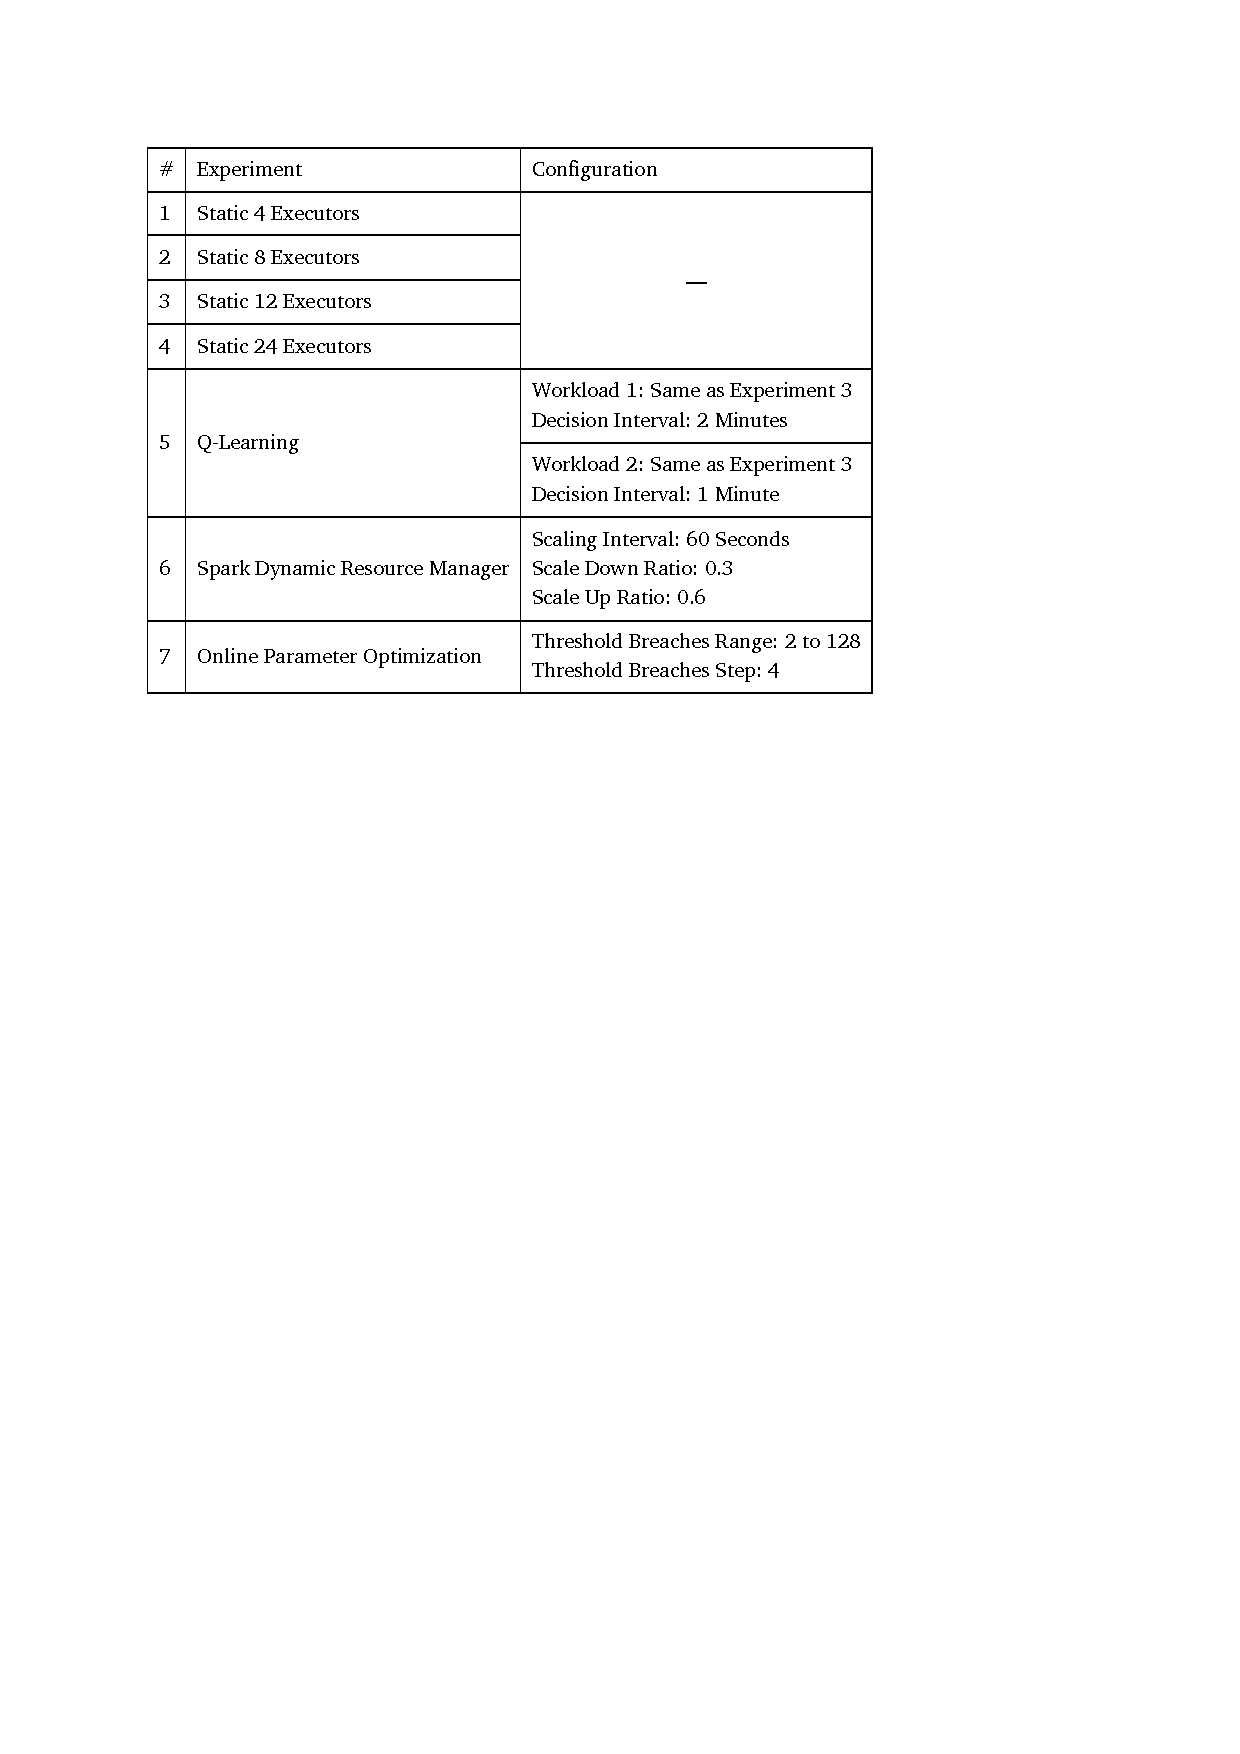
\includegraphics[clip,trim=2.4cm 17.9cm 6.1cm 2.5cm]{tables/ex9.pdf}
    \centering
    \caption{Overall Comparison Configuration Parameters}
    \label{eval:tab:ex9}
\end{table}

Note that, Spark Dynamic Resource Manager uses Equation~\ref{eval:e9:formula} to calculate a \emph{Ratio} value and then compares it to Scale-Up and Scale-Down ratio values obtained from configuration. In order to influence the behavior of this resource manager, batch duration should be changed. To make it fair, in all experiments the batch size is set to 10 seconds.
\begin{equation}
\text{Ratio} = \frac{\text{Average Latency of History Window}}{\text{Batch Size}}
\label{eval:e9:formula}
\end{equation}

For Q-Learning approach, two of the best cases from previous experiments were obtained. Also note that seven cases are evaluated in this experiment which makes it difficult to comprehend the detailed latency charts. Thus, they are removed. Figures~\ref{eval:f:e9:w1:lat-c} and~\ref{eval:f:e9:w2:lat-c} illustrate latency charts for both workloads. Figures~\ref{eval:f:e9:w1:exec-c} and~\ref{eval:f:e9:w2:exec-c} illustrates executor charts for both workloads.
\clearpage
\begin{figure}[H]
    \centering
    \begin{minipage}[h]{\linewidth}
        \centering
        \begin{gnuplot}[terminal=epslatex, terminaloptions=color colortext]
            set terminal epslatex size 17cm,11cm
            set key outside center top horizontal
            set datafile separator ';'
            set xr [0.5:7.5]
            set yr [0:420]
            set ytics 0,30 nomirror
            set y2r [0:420]
            set y2tics 0,30 nomirror
            set boxwidth 0.4 absolute
            set style fill empty
            set grid ytics lc rgb "#bbbbbb" lw 1 lt 0
            set grid xtics lc rgb "#bbbbbb" lw 1 lt 0
            unset xl
            set yl 'Latency (Seconds)'
            plot 'ex/final/w1/latency-c.csv' using 1:2:3:4:5:xticlabels(7) with candlesticks lc 'black' lw 4 t 'Min/Max/Percentiles',\
            '' using 1:6:6:6:6 with linespoints pt 5 lc 'black' lw 4 t 'Average'
        \end{gnuplot}
        \caption{Overall Comparison -- Workload 1 -- Latency}
        \label{eval:f:e9:w1:lat-c}
    \end{minipage}\hfil
    \begin{minipage}[h]{\linewidth}
        \centering
        \begin{gnuplot}[terminal=epslatex, terminaloptions=color colortext]
            set terminal epslatex size 17cm,11cm
            set key outside center top horizontal
            set datafile separator ';'
            set xr [0.5:7.5]
            set yr [0:390]
            set ytics 0,30 nomirror
            set y2r [0:390]
            set y2tics 0,30 nomirror
            set boxwidth 0.4 absolute
            set style fill empty
            set grid ytics lc rgb "#bbbbbb" lw 1 lt 0
            set grid xtics lc rgb "#bbbbbb" lw 1 lt 0
            unset xl
            set yl 'Latency (Seconds)'
            plot 'ex/final/w2/latency-c.csv' using 1:2:3:4:5:xticlabels(7) with candlesticks lc 'black' lw 4 t 'Min/Max/Percentiles',\
            '' using 1:6:6:6:6 with linespoints pt 5 lc 'black' lw 4 t 'Average'
        \end{gnuplot}
        \caption{Overall Comparison -- Workload 2 -- Latency}
        \label{eval:f:e9:w2:lat-c}
    \end{minipage}
\end{figure}
\clearpage
\begin{figure}[H]
    \centering
    \begin{minipage}[h]{\linewidth}
    \centering
    \begin{gnuplot}[terminal=epslatex, terminaloptions=color colortext]
        set terminal epslatex size 16cm,7.5cm
        set key outside center top horizontal
        set datafile separator ';'
        set xr [0.5:7.5]
        set yr [2:26]
        set y2r [2:26]
        set ytics 0,4 nomirror
        set y2tics 0,4 nomirror
        set boxwidth 0.4 absolute
        set style fill empty
        unset xl
        set grid ytics lc rgb "#bbbbbb" lw 1 lt 0
        set grid xtics lc rgb "#bbbbbb" lw 1 lt 0
        set yl 'Number of Executors'
        plot 'ex/final/w1/exec-c.csv' using 1:2:3:4:5:xticlabels(7) with candlesticks lc 'black' lw 4 t 'Min/Max/Percentiles',\
        '' using 1:6:6:6:6 with linespoints pt 5 lc 'black' lw 4 t 'Average' 
    \end{gnuplot}
    \caption{Overall Comparison -- Workload 1 -- Number of Executors}
    \label{eval:f:e9:w1:exec-c}
    \end{minipage}\hfil
    \begin{minipage}[h]{\linewidth}
    \centering
    \begin{gnuplot}[terminal=epslatex, terminaloptions=color colortext]
        set terminal epslatex size 16cm,7.5cm
        set key outside center top horizontal
        set datafile separator ';'
        set xr [0.5:7.5]
        set yr [2:26]
        set y2r [2:26]
        set ytics 0,4 nomirror
        set y2tics 0,4 nomirror
        set boxwidth 0.4 absolute
        set style fill empty
        unset xl
        set grid ytics lc rgb "#bbbbbb" lw 1 lt 0
        set grid xtics lc rgb "#bbbbbb" lw 1 lt 0
        set yl 'Number of Executors'
        plot 'ex/final/w2/exec-c.csv' using 1:2:3:4:5:xticlabels(7) with candlesticks lc 'black' lw 4 t 'Min/Max/Percentiles',\
        '' using 1:6:6:6:6 with linespoints pt 5 lc 'black' lw 4 t 'Average' 
    \end{gnuplot}
    \caption{Overall Comparison -- Workload 2 -- Number of Executors}
    \label{eval:f:e9:w2:exec-c}
    \end{minipage}
\end{figure}

As can be seen, from 8 to 12 executors the latency drops significantly. It can be concluded that to hit target latency -- which is 30 seconds in this case -- optimal number of executors is between 8 to 12. Note that, 12 executors is slightly better than 24 executors. This could be the result of extra network communication involved in case of 24 executors.

\section{Conclusion}

In this chapter Temporal Difference and Value Iteration algorithms were tested extensively. In most experiments even a small change leads to a significant change in Auto-Scaler's behavior. No generalized conclusion can be made based on the effect of configuration parameters. On one side under a proper configuration, it is able to achieve a better result than Spark and fixed number of executors. On the other side, the optimal configuration should be manually discovered by system administrator. Currently there is no \emph{systematic} approach available to find the optimal configuration. This has been left as future work.